\documentclass[]{book}
\usepackage{lmodern}
\usepackage{amssymb,amsmath}
\usepackage{ifxetex,ifluatex}
\usepackage{fixltx2e} % provides \textsubscript
\ifnum 0\ifxetex 1\fi\ifluatex 1\fi=0 % if pdftex
  \usepackage[T1]{fontenc}
  \usepackage[utf8]{inputenc}
\else % if luatex or xelatex
  \ifxetex
    \usepackage{mathspec}
  \else
    \usepackage{fontspec}
  \fi
  \defaultfontfeatures{Ligatures=TeX,Scale=MatchLowercase}
\fi
% use upquote if available, for straight quotes in verbatim environments
\IfFileExists{upquote.sty}{\usepackage{upquote}}{}
% use microtype if available
\IfFileExists{microtype.sty}{%
\usepackage{microtype}
\UseMicrotypeSet[protrusion]{basicmath} % disable protrusion for tt fonts
}{}
\usepackage[margin=1in]{geometry}
\usepackage{hyperref}
\hypersetup{unicode=true,
            pdftitle={Code-based, open-source software for teaching interactive data visualisation},
            pdfauthor={Shan-I Lee},
            pdfborder={0 0 0},
            breaklinks=true}
\urlstyle{same}  % don't use monospace font for urls
\usepackage{color}
\usepackage{fancyvrb}
\newcommand{\VerbBar}{|}
\newcommand{\VERB}{\Verb[commandchars=\\\{\}]}
\DefineVerbatimEnvironment{Highlighting}{Verbatim}{commandchars=\\\{\}}
% Add ',fontsize=\small' for more characters per line
\usepackage{framed}
\definecolor{shadecolor}{RGB}{248,248,248}
\newenvironment{Shaded}{\begin{snugshade}}{\end{snugshade}}
\newcommand{\KeywordTok}[1]{\textcolor[rgb]{0.13,0.29,0.53}{\textbf{{#1}}}}
\newcommand{\DataTypeTok}[1]{\textcolor[rgb]{0.13,0.29,0.53}{{#1}}}
\newcommand{\DecValTok}[1]{\textcolor[rgb]{0.00,0.00,0.81}{{#1}}}
\newcommand{\BaseNTok}[1]{\textcolor[rgb]{0.00,0.00,0.81}{{#1}}}
\newcommand{\FloatTok}[1]{\textcolor[rgb]{0.00,0.00,0.81}{{#1}}}
\newcommand{\ConstantTok}[1]{\textcolor[rgb]{0.00,0.00,0.00}{{#1}}}
\newcommand{\CharTok}[1]{\textcolor[rgb]{0.31,0.60,0.02}{{#1}}}
\newcommand{\SpecialCharTok}[1]{\textcolor[rgb]{0.00,0.00,0.00}{{#1}}}
\newcommand{\StringTok}[1]{\textcolor[rgb]{0.31,0.60,0.02}{{#1}}}
\newcommand{\VerbatimStringTok}[1]{\textcolor[rgb]{0.31,0.60,0.02}{{#1}}}
\newcommand{\SpecialStringTok}[1]{\textcolor[rgb]{0.31,0.60,0.02}{{#1}}}
\newcommand{\ImportTok}[1]{{#1}}
\newcommand{\CommentTok}[1]{\textcolor[rgb]{0.56,0.35,0.01}{\textit{{#1}}}}
\newcommand{\DocumentationTok}[1]{\textcolor[rgb]{0.56,0.35,0.01}{\textbf{\textit{{#1}}}}}
\newcommand{\AnnotationTok}[1]{\textcolor[rgb]{0.56,0.35,0.01}{\textbf{\textit{{#1}}}}}
\newcommand{\CommentVarTok}[1]{\textcolor[rgb]{0.56,0.35,0.01}{\textbf{\textit{{#1}}}}}
\newcommand{\OtherTok}[1]{\textcolor[rgb]{0.56,0.35,0.01}{{#1}}}
\newcommand{\FunctionTok}[1]{\textcolor[rgb]{0.00,0.00,0.00}{{#1}}}
\newcommand{\VariableTok}[1]{\textcolor[rgb]{0.00,0.00,0.00}{{#1}}}
\newcommand{\ControlFlowTok}[1]{\textcolor[rgb]{0.13,0.29,0.53}{\textbf{{#1}}}}
\newcommand{\OperatorTok}[1]{\textcolor[rgb]{0.81,0.36,0.00}{\textbf{{#1}}}}
\newcommand{\BuiltInTok}[1]{{#1}}
\newcommand{\ExtensionTok}[1]{{#1}}
\newcommand{\PreprocessorTok}[1]{\textcolor[rgb]{0.56,0.35,0.01}{\textit{{#1}}}}
\newcommand{\AttributeTok}[1]{\textcolor[rgb]{0.77,0.63,0.00}{{#1}}}
\newcommand{\RegionMarkerTok}[1]{{#1}}
\newcommand{\InformationTok}[1]{\textcolor[rgb]{0.56,0.35,0.01}{\textbf{\textit{{#1}}}}}
\newcommand{\WarningTok}[1]{\textcolor[rgb]{0.56,0.35,0.01}{\textbf{\textit{{#1}}}}}
\newcommand{\AlertTok}[1]{\textcolor[rgb]{0.94,0.16,0.16}{{#1}}}
\newcommand{\ErrorTok}[1]{\textcolor[rgb]{0.64,0.00,0.00}{\textbf{{#1}}}}
\newcommand{\NormalTok}[1]{{#1}}
\usepackage{longtable,booktabs}
\usepackage{graphicx,grffile}
\makeatletter
\def\maxwidth{\ifdim\Gin@nat@width>\linewidth\linewidth\else\Gin@nat@width\fi}
\def\maxheight{\ifdim\Gin@nat@height>\textheight\textheight\else\Gin@nat@height\fi}
\makeatother
% Scale images if necessary, so that they will not overflow the page
% margins by default, and it is still possible to overwrite the defaults
% using explicit options in \includegraphics[width, height, ...]{}
\setkeys{Gin}{width=\maxwidth,height=\maxheight,keepaspectratio}
\IfFileExists{parskip.sty}{%
\usepackage{parskip}
}{% else
\setlength{\parindent}{0pt}
\setlength{\parskip}{6pt plus 2pt minus 1pt}
}
\setlength{\emergencystretch}{3em}  % prevent overfull lines
\providecommand{\tightlist}{%
  \setlength{\itemsep}{0pt}\setlength{\parskip}{0pt}}
\setcounter{secnumdepth}{5}
% Redefines (sub)paragraphs to behave more like sections
\ifx\paragraph\undefined\else
\let\oldparagraph\paragraph
\renewcommand{\paragraph}[1]{\oldparagraph{#1}\mbox{}}
\fi
\ifx\subparagraph\undefined\else
\let\oldsubparagraph\subparagraph
\renewcommand{\subparagraph}[1]{\oldsubparagraph{#1}\mbox{}}
\fi

%%% Use protect on footnotes to avoid problems with footnotes in titles
\let\rmarkdownfootnote\footnote%
\def\footnote{\protect\rmarkdownfootnote}

%%% Change title format to be more compact
\usepackage{titling}

% Create subtitle command for use in maketitle
\newcommand{\subtitle}[1]{
  \posttitle{
    \begin{center}\large#1\end{center}
    }
}

\setlength{\droptitle}{-2em}
  \title{Code-based, open-source software for teaching interactive data
visualisation}
  \pretitle{\vspace{\droptitle}\centering\huge}
  \posttitle{\par}
  \author{Shan-I Lee}
  \preauthor{\centering\large\emph}
  \postauthor{\par}
  \date{}
  \predate{}\postdate{}


\usepackage{amsthm}
\newtheorem{theorem}{Theorem}[chapter]
\newtheorem{lemma}{Lemma}[chapter]
\theoremstyle{definition}
\newtheorem{definition}{Definition}[chapter]
\newtheorem{corollary}{Corollary}[chapter]
\newtheorem{proposition}{Proposition}[chapter]
\theoremstyle{definition}
\newtheorem{example}{Example}[chapter]
\theoremstyle{definition}
\newtheorem{exercise}{Exercise}[chapter]
\theoremstyle{remark}
\newtheorem*{remark}{Remark}
\newtheorem*{solution}{Solution}
\begin{document}
\maketitle

{
\setcounter{tocdepth}{1}
\tableofcontents
}
\chapter{Introduction}\label{introduction}

Tukey (1977) famously stated ``The greatest value of a picture is when
it \textbf{forces} us to notice what we never expected to see.'' (p vi).

Data visualisation uses graphics to gain further insight during data
exploration and confirmatory statistical analysis (Cook and Swayne
2007). In addition, \emph{interactive} data visualisation allows the
user to interact with graphical features in order to achieve fast and
flexible analysis (Unwin 2015). However Unwin (2015) highlights one of
the challenges of interactive data visualisation is in documenting the
interactions applied during analysis. The development of open-source,
code-based software, such as R packages, provides possible solutions to
address this issue. Hence it is of interest to research how effective
the current software tools are in implementing interactive techniques to
support the data analysis cycle. This helps to establish a focal set of
tools and techniques for teaching interactive data visualisation.

The first stage of this research entailed a survey on interactive
techniques and the range of open-source software currently available. A
literature review was undertaken to examine applications of interactive
techniques and identify commonly used techniques that should be
prioritised when teaching interactive data visualisation. The survey of
current software tools was then aimed towards evaluating their coverage
of these interactive techniques and the ease with which they could
achieve the interactivity. A set of software tools was identified and
used to explore the role of interactive data visualisation in the data
analysis cycle. This second stage of research applied interactive
techniques in exploratory data analysis of a dataset not previously
examined in the literature.

\section{Findings}\label{findings}

Different types of linked brushing, identification, subset selection and
tours, were found to be commonly used techniques in interactive data
visualisation. Utilising the \texttt{R} packages \textbf{plotly} and
\textbf{crosstalk} together, or in combination with \textbf{shiny}
software, provided a code-based, open-source approach towards applying
these interactive techniques. Awareness towards the limitations and code
efficiency of each software, enabled the efficient application of
interactive techniques to exploratory data analysis of a ``real''
dataset.

Applying interactive techniques to data analysis resulted in further
insight into underlying multivariate structures. For example tooltip
identification of outliers and linked brushing of individual and groups
of observations, capitalised on the multivariate views offered by
parallel coordinates plots. Furthermore interactive filtering helped to
reduce problems caused by overplotting and allowed the effect of sample
size on analysis to be explored.

Interactive techniques also helped to develop a deeper understanding of
abstract multivariate data analysis methods. Linked brushing between the
visual projections of a guided tour and its respective projection
pursuit index, prompted further exploration of the multidimensional data
space.

The benefits of utilising interactivity in data analysis outweighed the
effort required to implement the interactive techniques. Once sufficient
mastery of software was acquired, the interactive techniques could be
applied to new analysis in novel ways. The ease of applying interactive
techniques to gain deeper insight in analysis and a thorough
understanding of underlying processes, justifies teaching interactive
data visualisation to graduate students.

The following sections examine the different types of interactive
techniques and software tools available.

\chapter{Literature review of interactive techniques}\label{techniques}

The data analysis process described by Cook and Swayne (2007) provide a
structure and context for meaningful interactive data visualisation.
They emphasise the role of interactive techniques in identifying the
problem statement, preparing the data, enriching the exploratory and
quantitative analysis, and lastly in the presentation of findings. The
interactive techniques introduced by Cook and Swayne (2007) will form
the basis of discussion, intermixed with contributions from other
literature.

In their worked examples, Cook and Swayne (2007) primarily used the
interactive data visualisation software, \textbf{GGobi}. Although
\textbf{GGobi} is an open-source software, it is not code-based. The R
packages \textbf{plotly}, \textbf{crosstalk} and \textbf{shiny} provided
the interactivity required to create the examples in this section.
References to the strengths and weaknesses of these software will be
mentioned, but discussed in more detail in the Section \ref{software}.

The \textbf{crabs} dataset will be used to demonstrate interactive
techniques. The data consists of information on the \textbf{species}
(Blue or Orange), \textbf{sex} and five physical measurements of 200
Australian crabs: frontal lobe (\textbf{FL}), rear width (\textbf{RW}),
carapace length (\textbf{CL}), carapace width (\textbf{CW}) and body
depth (\textbf{BD}).

\begin{table}

\caption{\label{tab:crabs}A subset of the **crabs** dataset. The data consists of two categorical variables and five real-valued variables.}
\centering
\begin{tabular}[t]{lllrrrrr}
\toprule
  & species & sex & FL & RW & CL & CW & BD\\
\midrule
1 & B & M & 8.1 & 6.7 & 16.1 & 19.0 & 7.0\\
2 & B & M & 8.8 & 7.7 & 18.1 & 20.8 & 7.4\\
51 & B & F & 7.2 & 6.5 & 14.7 & 17.1 & 6.1\\
52 & B & F & 9.0 & 8.5 & 19.3 & 22.7 & 7.7\\
101 & O & M & 9.1 & 6.9 & 16.7 & 18.6 & 7.4\\
\addlinespace
102 & O & M & 10.2 & 8.2 & 20.2 & 22.2 & 9.0\\
151 & O & F & 10.7 & 9.7 & 21.4 & 24.0 & 9.8\\
152 & O & F & 11.4 & 9.2 & 21.7 & 24.1 & 9.7\\
\bottomrule
\end{tabular}
\end{table}

\section{Linked brushing}\label{linked-brushing}

The interactive technique of linked brushing involves using the mouse to
select one or more graphical features, which then prompts related
features in the same plot and/or other plots to be highlighted in the
same colour (Cook and Swayne 2007). There are different types of linked
brushing, depending on the linking rule used. The most basic form of
linking is one-to-one. Figures and demonstrate linked brushing between a
plot representing the two categorical variables of the \textbf{crabs}
dataset and a scatterplot of the carapace length and rear width. The
linking can be initiated by brushing points in either plot. The brushed
regions are marked by a dashed boundary. Figure also demonstrates
persistent brushing, where the results from previous selections are
retained in subsequent brushing. Cases linked by different ``brushes''
are also distinguished by colour in Figure .

\begin{figure}[center]
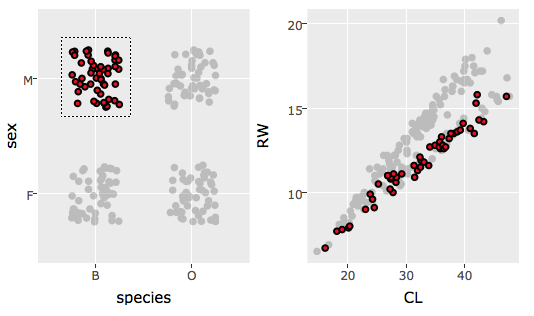
\includegraphics[width=700px]{files/one2one} \caption{The group of points representing male crabs of the Blue species is brushed to link with their carapace length and rear width measurements in the scatterplot.}\label{fig:one2one}
\end{figure}

\begin{figure}[center]
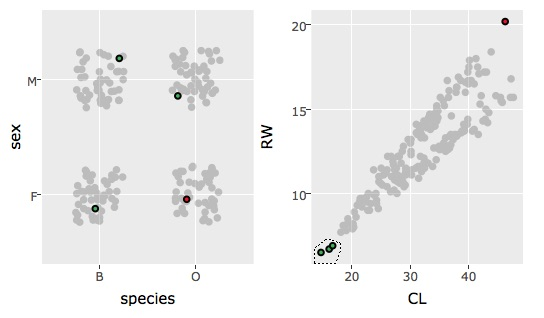
\includegraphics[width=700px]{files/one2one2} \caption{An example of one-to-one linking and persistent brushing. The crab with the largest rear width measurement was first brushed, followed by the group of three smaller crabs. The sex and species of the four crabs are highlighted corresponding to the colours used in the brushing.}\label{fig:one2one2}
\end{figure}

Instead of linking by case, a categorical variable can also be used to
define the linking rule. This results in all members of the same level
being highlighted, once one member is brushed (Cook and Swayne 2007).
Gender is used as the linking rule in Figure \ref{fig:catbrush} so that
brushing one female crab links to highlighting points for all female
crabs in the same plot.

\begin{figure}[center]
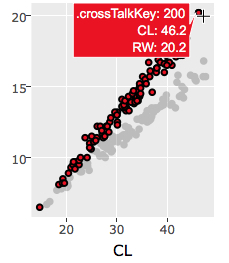
\includegraphics[width=700px]{files/catbrush} \caption{Categorical brushing where brushing one female crab highlights all points representing female crabs.}\label{fig:catbrush}
\end{figure}

The query resulting from the categorical brushing in Figure
\ref{fig:catbrush} can also be achieved by brushing on a bar chart for
the gender of the crabs and linking to the points in the scatterplot
shown. For web-based software, brushing on visuals representing
aggregated data, such as bar plots, is more challenging than linking by
case (RStudio 2017a). Although not impossible, the user needs to
explicitly communicate details of the aggregation. This becomes more
challenging when continuous variables are aggregated, or mosaic plots
involving several categorical variables are used. The web-based R
package \textbf{animint} attempts to make the implementation of
aggregate brushing easier, but it is currently limited to discrete
values and does not incorporate the flexibility of brushing by case
(Hocking 2017).

Linked brushing within a parallel coordinates plot (PCP) provides an
example of \emph{m}-to-\emph{n} linking. A PCP displays multiple
variables in a single plot by using parallel axes, rather than being
restricted to two orthogonal axes, as in a scatterplot. Variable values
on adjacent axes belonging to the same observation are joined by line
segments. The parallel axes are typically scaled individually to
maximise use of space on the plot, but global values can be used to
establish a common scale for all axes as well (Unwin 2015). Figure
\ref{fig:m2nuni} uses five vertical axes, scaled individually to the
range of each physical measurement recorded in the \textbf{crabs}
dataset. The edges joining the nodes are relatively horizontal which
suggests positive correlation between adjacent variables. Brushing the
highest value on the \textbf{RW} axis links together the five physical
measurements of the crab with the largest rear width. Hence linking
together \emph{m} nodes with \emph{n} edges.

\begin{figure}[htbp]
\centering
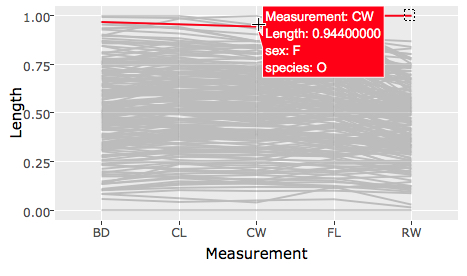
\includegraphics{files/m2n_uni.jpg}
\caption{\label{fig:m2nuni}An example of m-to-n linking and identification.
The five physical measurements of the crab with the largest rear width
are linked together by brushing. Tooltips identify the crab as a female
Orange crab.}
\end{figure}

\section{Identification}\label{identification}

Identification using tooltips is also demonstrated in Figure
\ref{fig:m2nuni}. Labels containing variable values appear as the mouse
``hovers'' over graphical features representing the values. Theus
(2017b) refers to this technique as ``querying'' the data and applies it
to quickly answer basic questions during exploratory data analysis.

\section{Scaling}\label{scaling}

The use of different scales in visual displays can reveal different
features of the data (Cook and Swayne 2007). Theus (2017b) uses a PCP to
analyse the time taken by cyclists to finish each stage of the 2013 Tour
de France competition. He uses the \textbf{Mondrian} software's
graphical user interface (GUI) to interactively change the scaling on
the parallel axes to make a variety of comparisons between different
stages of the race and the progress of competitors.

Figure \ref{fig:m2nglobal} displays the same data as in Figure
\ref{fig:m2nuni}, but uses the overall range of the five physical
measurements to apply a common scale to the parallel axes. The crab with
the largest rear width is again brushed and identified. The change in
scaling makes the correlation between variables more difficult to see in
the figure below and the nodes even harder to brush individually, than
the previous plot.

\begin{figure}[htbp]
\centering
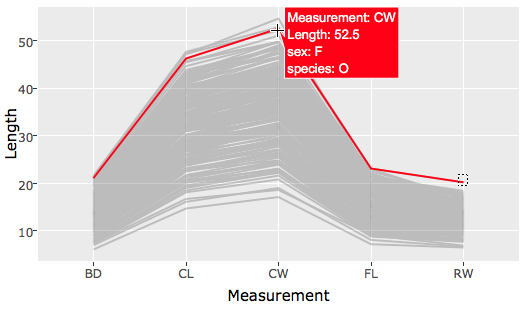
\includegraphics{files/m2n_global.jpg}
\caption{\label{fig:m2nglobal}Applying a global scale hides the correlation
between variables and causes the plot to become easily overplotted.}
\end{figure}

Being able to zoom in or out of a plot provides another mode of
interactive scaling. This can be particularly useful for viewing busy
regions of a plot (Cook and Swayne 2007). By default, all interactive
plots created using the \textbf{plotly} package have zoom and pan
controls that are accessible via its hovering menu of interactive
techniques, at the top of the plot (Sievert 2017).

\section{Line segments}\label{line-segments}

Line segments are essential to visualisations involving longitudinal
data and are often used to represent models (Cook and Swayne 2007).
Wickham, Cook, and Hofmann (2015) analysed a clustering algorithm by
creating a dynamic visualisation using grid lines to represent models
generated at each iteration. In network graphs, line segements define
characteristics of connections between nodes. For example the weight of
line segments between nodes (people) in a social network can reflect the
frequency of exchanges between two people. Hence being able to brush and
query line segments would be useful when applying interactive data
visualisation to network analysis (Cook and Swayne 2007).

Unlike \textbf{GGobi}, the web-based software tools examined were unable
to brush lines. The linked brushing previously demonstrated in the PCP
was achieved by brushing a node on the \textbf{RW} variable's axis.
Similarly, the \textbf{Mondrian} software limits brushing on a PCP to
the nodes (Theus 2017a). Linked brushing on dendrograms, using the
\textbf{plotly} package is also restricted to brushing the nodes
(Sievert 2016).

\section{Subset selection}\label{subset-selection}

Subset selection involves using only a portion of the data for
visualisation and/or analysis. This technique can help elleviate the
computational strain and overplotting caused by large datasets (Cook and
Swayne 2007). The \textbf{shiny} software provides different interactive
input controls for subsetting data before mapping to graphical features
or performing statistical analysis. Furthermore since interactive
visuals created with \textbf{shiny} are connected to an active R
session, it allows for analysis to be dynamically updated (RStudio
2017c). Without access to statistical software during interactive subset
selection, only a filtering of pre-defined visual output is possible
(Seivert 2017).

\section{Tours: A dynamic multivariate visual
representation}\label{tours-a-dynamic-multivariate-visual-representation}

Wickham et al. (2011) highlight tours as essential for gaining insight
into the structures underlying real-valued multivariate data. A tour is
an animation consisting of static low-dimensional projections of
high-dimensional data space. The projections to include in a tour can be
manually determined, randomly chosen, or guided by algorithms, such as
projection pursuits (Cook and Swayne 2007). The latter two options are
referred to as grand tours and guided tours, respectively. Wickham et
al. (2011) define guided tours as a ``dynamic form of projection
pursuit'' (p.4) and highlight the value of being able to examine views
of local maximal, in addition to the final ``solution''.

The \textbf{crabs} dataset was examined by Venables and Ripley (2002)
using principal component analysis (PCA) on the log values of the five
physical measurements. PCA reveals interesting multivariate structures
by finding projections of the data that show maximal variability
(Venables and Ripley 2002). Hence principal components are commonly used
to provide a starting basis for interactive tours (Wickham et al. 2011).

Figure @ref(fig:tour\_init) shows a two-dimensional guided tour of the
five dimensional space, spanned by the real-valued variables of the
\textbf{crabs} dataset. On the right of the tour plot, line segments are
used to represent the orientation of the projection with respect to the
original variables. The R package \textbf{tourr}, enables projection
pursuit indices and geodesic interpolation between projections, to be
applied. The interpolation between projections is a stochastic process,
hence the views observed will vary between tours (Wickham et al. 2011).
The second and third principal components of the log values were
identified by Venables and Ripley (2002) as almost separating the four
sex-species crab classes. The projection defined by the principal
components indicated a sparse distribution at the centre, hence the
choice in using the ``holes'' projection pursuit index. This projection
of the data was used as the starting basis for the guided tour to
further explore the ``neighbourhood'' identified by Venables and Ripley
(2002).

\begin{figure}[htbp]
\centering
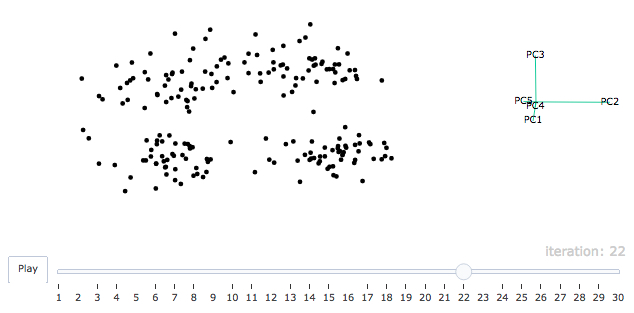
\includegraphics{files/tour.jpg}
\caption{(\#fig:tour\_init)A 2D guided tour of the five-dimensional
space spanned by the real-valued variables of the crabs dataset.}
\end{figure}

A slight improvement on separating the four sex-species crab classes is
possible. Figure @ref(fig:tour\_brush) shows a projection from the tour
with persistent one-to-one linked brushing applied.

\begin{figure}[htbp]
\centering
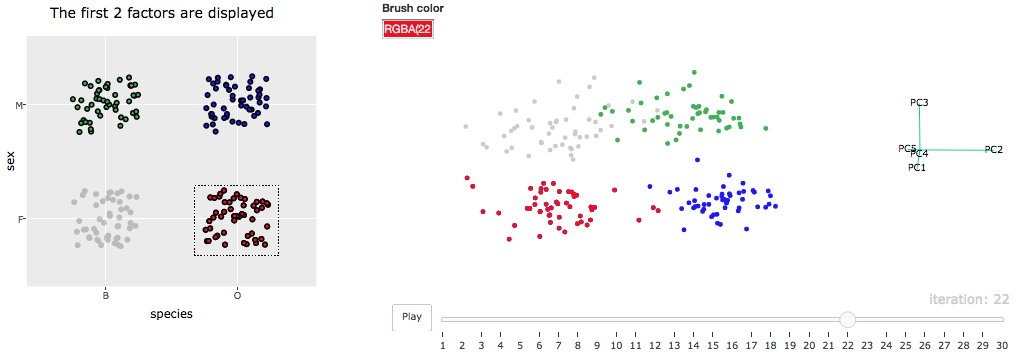
\includegraphics{files/tour_brush.jpg}
\caption{(\#fig:tour\_brush)A projection from a guided tour with
persistent brushing applied across projections.}
\end{figure}

Cook and Swayne (2007) demonstrate how persistent linked brushing
between projections of a tour, enables graphical approaches towards
supervised classification and cluster analysis. Although the animation
required for tours can be achieved in \textbf{shiny}, a ``spin and
brush'' technique cannot be facilitated due to each projection being
independently rendered. In Figure @ref(fig:tour\_init) it is possible to
pause the animation, brush the tour plot and then continue the tour,
since \textbf{crosstalk} was used to provide the linking between the
data for the projections.

\chapter{A survey of software tools}\label{software}

The demonstrations of interactive techniques in Section
\ref{techniques}, show that a code-based approach towards achieving the
scope of techniques possible in \textbf{GGobi}, requires the use of more
than one software. This section compares the ease of application,
development progress and coverage of interactive techniques, for a range
of open-source, code-based software tools. A set of key software tools
will be identified and discussed in more detail.

\section{Types of interactive software}\label{types}

Lang and Swayne (2001) describe two types of interactive data
visualisation software, those with a direct manipulation graphical
environment and those driven by a command-line interface. \textbf{GGobi}
and \textbf{Mondrian} are examples of software programmes that have a
GUI for direct manipulation. GUI environments provide immediate response
to user actions, but without technical knowledge of the underlying
low-level language, it is difficult to modify or extend these types of
software (Lang and Swayne 2001). On the other hand, command-line
interfaces, such as R, not only allow modification of existing
capabilities, but also the creation of new functions. Furthermore the R
software provides access to a vast range of techniques and tools for
statistical analysis (Unwin 2015).

R packages for interactive data visualisation aim to reap the benefits
of direct manipulation, the extensibility of a scripting language and
the statistical power of the R environment. The package \textbf{rggobi}
connects the \textbf{GGobi} GUI with R, to enable complex interactive
graphical analyses that would be difficult, if not impossible, to carry
out without a command-line interface (Lawrence et al. 2009). Meanwhile
packages like \textbf{plotly}, \textbf{crosstalk} and \textbf{shiny},
utilise the interactive graphics provided by the web, alongside the
statistical functions accessible in R. The use of web browsers minimises
the software requirements for utilising these packages. Unwin (2015)
highlights that the shift towards web-based software helps to make
sharing and presenting analyses from interactive data visualisations
easier. In contrast \textbf{rggobi} is dependent on the installation of
\textbf{GGobi} and the specific software required for building the
\textbf{GGobi} GUI. Consequently the ease of access to \textbf{rggobi}
is at a disadvantage to the other R packages.

Other R packages for interactive data visualisation include
\textbf{trelliscopejs} and \textbf{animint}. Like \textbf{plotly} these
software build on the comprehensive graphing system provided by the R
package \textbf{ggplot2}. By adding interactive functions,
\textbf{trelliscopejs}, \textbf{animint} and \textbf{plotly}, convert
static \textbf{ggplot2} objects into web-based interactive plots. The
\textbf{trelliscopejs} package focuses on adding interactive techniques
to trellis plots. Hafen (2017) describes \textbf{trelliscopejs} as
enabling ``interactivity for free'' and emphasises that adding
interactivity should require little time and effort beyond that needed
to create the static plot. The design behind \textbf{animint} reflects a
similar sentiment but enables interactivity for a wider range of plot
types. It enables linked brushing by introducing additional arguments to
the mapping system used in \textbf{ggplot2}. However currently this
interactive technique can only be activated by conditioning on
categorical or discrete variables (Hocking 2017). Furthermore all
calculations are pre-computed before plot compilation and hence genuine
``real-time'' analysis in response to interactivity, is not possible.
The \textbf{plotly} package shares this limitation, but it enables more
flexible brushing and a wider variety of linking, when paired with other
software. Furthermore \textbf{plotly} appears to be further along in its
development, unlike \textbf{trelliscopejs} and \textbf{animint}, it is
already available on the Comprehensive R Archive Network (CRAN). For the
purposes of teaching, the availability of \textbf{plotly} on CRAN
provides ease of installation and documentation for support.

Instead of adding interactive components to \textbf{ggplot2} objects,
the \textbf{ggvis} package shares a similar syntax, inspired by the
grammar of graphics (RStudio 2017b). The interactive features enabled by
\textbf{ggvis} are similar to those available through \textbf{shiny}.
For example the \texttt{input\_slider()} function in \textbf{ggvis}
creates an interactive slider equivalent to the functionality of
\textbf{shiny}'s \texttt{sliderInput()}. Both software tools need to be
connected to a R session in order for the interactive plots to be
active. When applying interactive data visualisation for exploration and
early stages of analysis, this is particularly useful because it allows
the statistical analysis in R to respond directly to interactive inputs
from visuals (RStudio 2017b). However for the purpose of presentation,
interactive graphics created using \textbf{ggvis} or \textbf{shiny}
would need to be hosted on a server. In contrast, interactive
\textbf{plotly} and \textbf{crosstalk} visuals are easy to share as a
standalone HTML (Seivert 2017). In comparision to \textbf{shiny}, more
aspects of \textbf{ggvis} are still underdevelopment and hence there may
be significant changes to its current interfaces (RStudio 2017b).
Furthermore, \textbf{shiny} has the extra advantage of being compatible
with a range of other software, such as \textbf{plotly} and
\textbf{crosstalk}, whilst providing similar interactive functionality
as \textbf{ggvis}.

\section{A set of software tools}\label{a-set-of-software-tools}

Ease of application, development progress and coverage of interactive
techniques were the main criterion used to identify \textbf{plotly},
\textbf{crosstalk} and \textbf{shiny} as a focal set of software tools
for teaching interactive data visualisation.

\subsection{Coverage of interactive
techniques}\label{coverage-of-interactive-techniques}

The interactive techniques discussed in Section \ref{techniques} are not
intended to be exhaustive, but they provide a powerful toolbox for
applying interactive data visualisation (Cook and Swayne 2007). The
tables below summarise how well the set of interactive software tools,
\textbf{shiny}, \textbf{plotly} and \textbf{crosstalk}, implement the
interactive techniques discussed.

Table \ref{tab:techniques} examines the coverage of each package as a
standalone software. For example, unless \textbf{crosstalk} is combined
with \textbf{shiny} it does not have access to an active R session.
Although this feature is not an interactive technique, it has been
included in Table \ref{tab:techniques} since having access to
statistical software enables a two-way workflow between data analysis
and plot interaction (Wickham et al. 2009). As previously discussed,
this enables the implementation of techniques like subset selection, but
affects the ease of sharing interactive visualisations.

\begin{longtable}[]{@{}lccccc@{}}
\caption{\label{tab:techniques} Coverage of interactive techniques by
\textbf{shiny}, \textbf{plotly} and \textbf{crosstalk}
software.}\tabularnewline
\toprule
\begin{minipage}[b]{0.11\columnwidth}\raggedright\strut
R Package\strut
\end{minipage} & \begin{minipage}[b]{0.17\columnwidth}\centering\strut
ActiveR session\strut
\end{minipage} & \begin{minipage}[b]{0.16\columnwidth}\centering\strut
TooltipIdentification\strut
\end{minipage} & \begin{minipage}[b]{0.10\columnwidth}\centering\strut
Scaling\strut
\end{minipage} & \begin{minipage}[b]{0.18\columnwidth}\centering\strut
Subset selection\strut
\end{minipage} & \begin{minipage}[b]{0.11\columnwidth}\centering\strut
Animation(for tours)\strut
\end{minipage}\tabularnewline
\midrule
\endfirsthead
\toprule
\begin{minipage}[b]{0.11\columnwidth}\raggedright\strut
R Package\strut
\end{minipage} & \begin{minipage}[b]{0.17\columnwidth}\centering\strut
ActiveR session\strut
\end{minipage} & \begin{minipage}[b]{0.16\columnwidth}\centering\strut
TooltipIdentification\strut
\end{minipage} & \begin{minipage}[b]{0.10\columnwidth}\centering\strut
Scaling\strut
\end{minipage} & \begin{minipage}[b]{0.18\columnwidth}\centering\strut
Subset selection\strut
\end{minipage} & \begin{minipage}[b]{0.11\columnwidth}\centering\strut
Animation(for tours)\strut
\end{minipage}\tabularnewline
\midrule
\endhead
\begin{minipage}[t]{0.11\columnwidth}\raggedright\strut
Shiny\strut
\end{minipage} & \begin{minipage}[t]{0.17\columnwidth}\centering\strut
Yes\strut
\end{minipage} & \begin{minipage}[t]{0.16\columnwidth}\centering\strut
\strut
\end{minipage} & \begin{minipage}[t]{0.10\columnwidth}\centering\strut
\strut
\end{minipage} & \begin{minipage}[t]{0.18\columnwidth}\centering\strut
Yes(via \texttt{Inputs})\strut
\end{minipage} & \begin{minipage}[t]{0.11\columnwidth}\centering\strut
Yes\strut
\end{minipage}\tabularnewline
\begin{minipage}[t]{0.11\columnwidth}\raggedright\strut
Plotly\strut
\end{minipage} & \begin{minipage}[t]{0.17\columnwidth}\centering\strut
\strut
\end{minipage} & \begin{minipage}[t]{0.16\columnwidth}\centering\strut
Yes\strut
\end{minipage} & \begin{minipage}[t]{0.10\columnwidth}\centering\strut
Yes\strut
\end{minipage} & \begin{minipage}[t]{0.18\columnwidth}\centering\strut
Limited tofiltering views\strut
\end{minipage} & \begin{minipage}[t]{0.11\columnwidth}\centering\strut
Yes\strut
\end{minipage}\tabularnewline
\begin{minipage}[t]{0.11\columnwidth}\raggedright\strut
Crosstalk\strut
\end{minipage} & \begin{minipage}[t]{0.17\columnwidth}\centering\strut
\strut
\end{minipage} & \begin{minipage}[t]{0.16\columnwidth}\centering\strut
\strut
\end{minipage} & \begin{minipage}[t]{0.10\columnwidth}\centering\strut
\strut
\end{minipage} & \begin{minipage}[t]{0.18\columnwidth}\centering\strut
Limited tofiltering views\strut
\end{minipage} & \begin{minipage}[t]{0.11\columnwidth}\centering\strut
Yes\strut
\end{minipage}\tabularnewline
\bottomrule
\end{longtable}

Linked brushing is summarised separately in Table \ref{tab:brushing}
since there is a variety of ways to define linking rules. Furthermore
the implementation of linked brushing generally requires the packages to
be combined. Enabling dynamic tours also require the additional
\textbf{tourr} package.

\begin{longtable}[]{@{}lccccc@{}}
\caption{\label{tab:brushing} Implementing linked brushing using
combinations of \textbf{shiny}, \textbf{plotly} and \textbf{crosstalk}
software.}\tabularnewline
\toprule
\begin{minipage}[b]{0.11\columnwidth}\raggedright\strut
R Packages\strut
\end{minipage} & \begin{minipage}[b]{0.20\columnwidth}\centering\strut
Linkone-to-one\strut
\end{minipage} & \begin{minipage}[b]{0.13\columnwidth}\centering\strut
Categoricalbrushing\strut
\end{minipage} & \begin{minipage}[b]{0.12\columnwidth}\centering\strut
Persistentbrushing\strut
\end{minipage} & \begin{minipage}[b]{0.13\columnwidth}\centering\strut
Brush lines\strut
\end{minipage} & \begin{minipage}[b]{0.13\columnwidth}\centering\strut
Spin and brush(for tours)\strut
\end{minipage}\tabularnewline
\midrule
\endfirsthead
\toprule
\begin{minipage}[b]{0.11\columnwidth}\raggedright\strut
R Packages\strut
\end{minipage} & \begin{minipage}[b]{0.20\columnwidth}\centering\strut
Linkone-to-one\strut
\end{minipage} & \begin{minipage}[b]{0.13\columnwidth}\centering\strut
Categoricalbrushing\strut
\end{minipage} & \begin{minipage}[b]{0.12\columnwidth}\centering\strut
Persistentbrushing\strut
\end{minipage} & \begin{minipage}[b]{0.13\columnwidth}\centering\strut
Brush lines\strut
\end{minipage} & \begin{minipage}[b]{0.13\columnwidth}\centering\strut
Spin and brush(for tours)\strut
\end{minipage}\tabularnewline
\midrule
\endhead
\begin{minipage}[t]{0.11\columnwidth}\raggedright\strut
Plotly+Shiny\strut
\end{minipage} & \begin{minipage}[t]{0.20\columnwidth}\centering\strut
\strut
\end{minipage} & \begin{minipage}[t]{0.13\columnwidth}\centering\strut
Easier\strut
\end{minipage} & \begin{minipage}[t]{0.12\columnwidth}\centering\strut
Yes\strut
\end{minipage} & \begin{minipage}[t]{0.13\columnwidth}\centering\strut
\strut
\end{minipage} & \begin{minipage}[t]{0.13\columnwidth}\centering\strut
\strut
\end{minipage}\tabularnewline
\begin{minipage}[t]{0.11\columnwidth}\raggedright\strut
Plotly+Crosstalk\strut
\end{minipage} & \begin{minipage}[t]{0.20\columnwidth}\centering\strut
Easier\strut
\end{minipage} & \begin{minipage}[t]{0.13\columnwidth}\centering\strut
\strut
\end{minipage} & \begin{minipage}[t]{0.12\columnwidth}\centering\strut
Yes\strut
\end{minipage} & \begin{minipage}[t]{0.13\columnwidth}\centering\strut
\strut
\end{minipage} & \begin{minipage}[t]{0.13\columnwidth}\centering\strut
Yes\strut
\end{minipage}\tabularnewline
\bottomrule
\end{longtable}

The \textbf{plotly} package provides a starting point that enables the
application of a variety of interactive techniques. The default settings
for a \textbf{plotly} object allow for tooltip identification, scaling
and filtering via the legend (where applicable). Interactive plots can
be created by either converting static \textbf{ggplot2} plots to
\textbf{plotly} objects, or directly using the \texttt{plot\_ly()}
function. The \textbf{plotly} syntax is conveniently similar to
\textbf{ggplot2}. Although \textbf{ggplot2} provides a more extensive
system of graphics, creating interactive visualisations using
\texttt{plot\_ly()} utilises the \textbf{plotly.js} library more
directly (Sievert 2017).

Combining \textbf{plotly} with \textbf{crosstalk} introduces the key
interactive technique of brushing to link multiple plots. Linked
brushing can also be achieved by using \textbf{plotly} and
\textbf{shiny} together, but the \texttt{SharedData} environment of the
\textbf{crosstalk} package allows default one-to-one linked brushing
between any plots sharing the same environment. Hence little additional
code is required to implement basic linked brushing when using
\textbf{crosstalk}. In contrast, using \textbf{shiny} involves writing
code to ``manually'' subset the selected data using the reactive output
from the plot interaction. This enables categorical brushing, as
demonstrated in Figure \ref{fig:catbrush}. A similar approach can be
applied to achieve brushing on aggregated data using \textbf{plotly} and
\textbf{shiny}, but more code and effort would be required as the
complexity of area plots increase.

The \textbf{crosstalk} package takes advantage of the variety of
web-based graphics that is available by providing interactivity between
HTML widgets. It is intended to be used with other software, but the
\textbf{crosstalk} package is not appropriate for use with large
datasets and currently supports only the interactive techniques of
linked brushing and filtering views (RStudio 2017a).

In the set of software tools, the \textbf{shiny} package provides a
connection to R when the interactive data visualisation requires it.
However enabling analysis that responds to interactivity comes at a
cost. Compared to the other two packages, more code and effort is
generally required to set up the three-component structure behind
\textbf{shiny} apps. Consequently the learning curve is also greater,
but \textbf{shiny} is well supported with online tutorials and
exemplars.\footnote{See \url{http://shiny.rstudio.com/tutorial/} for
  resources.}

\chapter{The role of interactive visualisation in data
analysis}\label{the-role-of-interactive-visualisation-in-data-analysis}

This section examines the use of interactive visualisation techniques in
exploratory data analysis on the performance of New Zealand schools in
the National Certificate of Educational Achievement (NCEA) in 2016. The
role of interactive techniques in enhancing analysis and gaining further
insight than static plots, will be be highlighted and demonstrated
through worked examples.

\begin{boxed}
Key findings with regards to the use of interactive techniques in data
analysis, or the teaching of interactive data visualisation, will be
noted explicitly as they are demonstrated using the NCEA dataset.
\end{boxed}

\section{The NCEA dataset}\label{the-ncea-dataset}

Data on the achievement rates of schools across the four NCEA
qualification levels, Level One, Two, Three (L1, L2, L3) and University
Entrance (UE), were obtained from the New Zealand Qualifications
Authority (NZQA) website.\footnote{Data retrieved from
  \url{http://www.nzqa.govt.nz/assets/Studying-in-NZ/Secondary-school-and-NCEA/stats-reports/2016/Qualification-Statistics-School-2016-29032017.csv}.}
Students need to demonstrate sufficient mastery of standards at each
respective NCEA level in order to be awarded the qualification. The UE
qualification differs from L3, in that the standards achieved need to be
from ``university endorsed'' Level Three subjects, and specific
requirements for literacy and numeracy must be met.

Information on the school decile, region and a ``small'' cohort warning,
were also provided in the data. The decile rating is a measure of the
general income level of the families of students attending the school.
The socio-economic background of students increases as the decile
increase from one to ten. A handful of schools have a decile rating of
zero, due to unique circumstances that make them exempt from the
socio-economic measure. The achievement rate of a school for each
qualification level was quantified in a few ways. The achievement
indicator chosen for this analysis was the proportion of students at the
school who were successful in obtaining the qualification level, given
that they were entered in enough standards to have the opportunity to
earn the qualification in the 2016 school year. This is referred to as
the ``Current Year Achievement Rate'' for the ``Participating Cohort''
by the NZQA.\footnote{For more details provided by the NZQA, see
  \url{http://www.nzqa.govt.nz/assets/Studying-in-NZ/Secondary-school-and-NCEA/stats-reports/NZQA-Secondary-Statistics-Consolidated-Data-Files-Short-Guide.pdf}).}

After tidying the data retrieved from the NZQA website, the
\textbf{NCEA} dataset consists of four real-valued variables, the
achievement rates and one categorical variable for the decile rating of
the school. Only schools with achievement indicators across all four
qualification levels were retained, thus reducing the dataset to 408
schools from around New Zealand. The focus of analysis will be on its
subset of 91 Auckland schools, but the New Zealand dataset of 408
schools will be used to demonstrate how interactive techniques can aid
graphical analysis when observations increase. The sensitivity of
analysis to samples size for the New Zealand schools dataset will also
be explored interactively.

Analysis of data for the Auckland subset will be the focus because it is
less affected by the unreliability of small sample sizes. Auckland has
many of the larger schools since it is the most populated city in New
Zealand. The first few observations from the dataset of 91 schools in
the Auckland region are shown in Table \ref{tab:akl}.

\begin{table}

\caption{\label{tab:akl}The first few observations from the **NCEA** dataset. The data consists of four real-valued variables and one categorical variable.}
\centering
\begin{tabular}[t]{lrrrrl}
\toprule
  & L1 & L2 & L3 & UE & Decile\\
\midrule
Al-Madinah School & 0.889 & 1.000 & 1.000 & 0.640 & 2\\
Albany Senior High School & 0.905 & 0.904 & 0.882 & 0.701 & 10\\
Alfriston College & 0.659 & 0.651 & 0.563 & 0.369 & 2\\
\bottomrule
\end{tabular}
\end{table}

\section{Static visual analysis}\label{static-visual-analysis}

A question that naturally arises from the NCEA data is whether a
school's performance is related to its decile rating. Using graphics in
data analysis entails considering multiple views of the data, starting
with simple low dimensional representations before examining complex
multivariate structures (Unwin 2015, Cook and Swayne (2007)).

The pairs plot in Figure \ref{fig:pairs} shows the achievement rates at
L1, L2 and L3 have a weak relationship with decile rating, but the
positive correlation is strong at UE. There appears to be an increasing
``lower bound'' to achievement rates for L1, L2 and L3, as decile
increases, but there is a lot of scatter above this boundary. In the
bivariate scatterplots we can also see the spread of achievement rates
varying across decile groups. The variation in achievement rates
decreases as the decile increases (from one), across the L1, L2 and L3
qualification levels. We can see many schools approaching the maximum
100\% achievement rate, for L1, L2 and L3, hence it is not surprising to
see their univariate distributions are skewed to the left in Figure
\ref{fig:hists}. The distribution of achievement rates for UE is less
skewed and hints at two possible groupings. Furthermore performance
across the qualification levels appear to be positively correlated,
especially between L1 and L2. Hence the low-dimensional plots indicate
non-normality, unequal spread between groups and multicollinearity.

\begin{figure}[htbp]
\centering
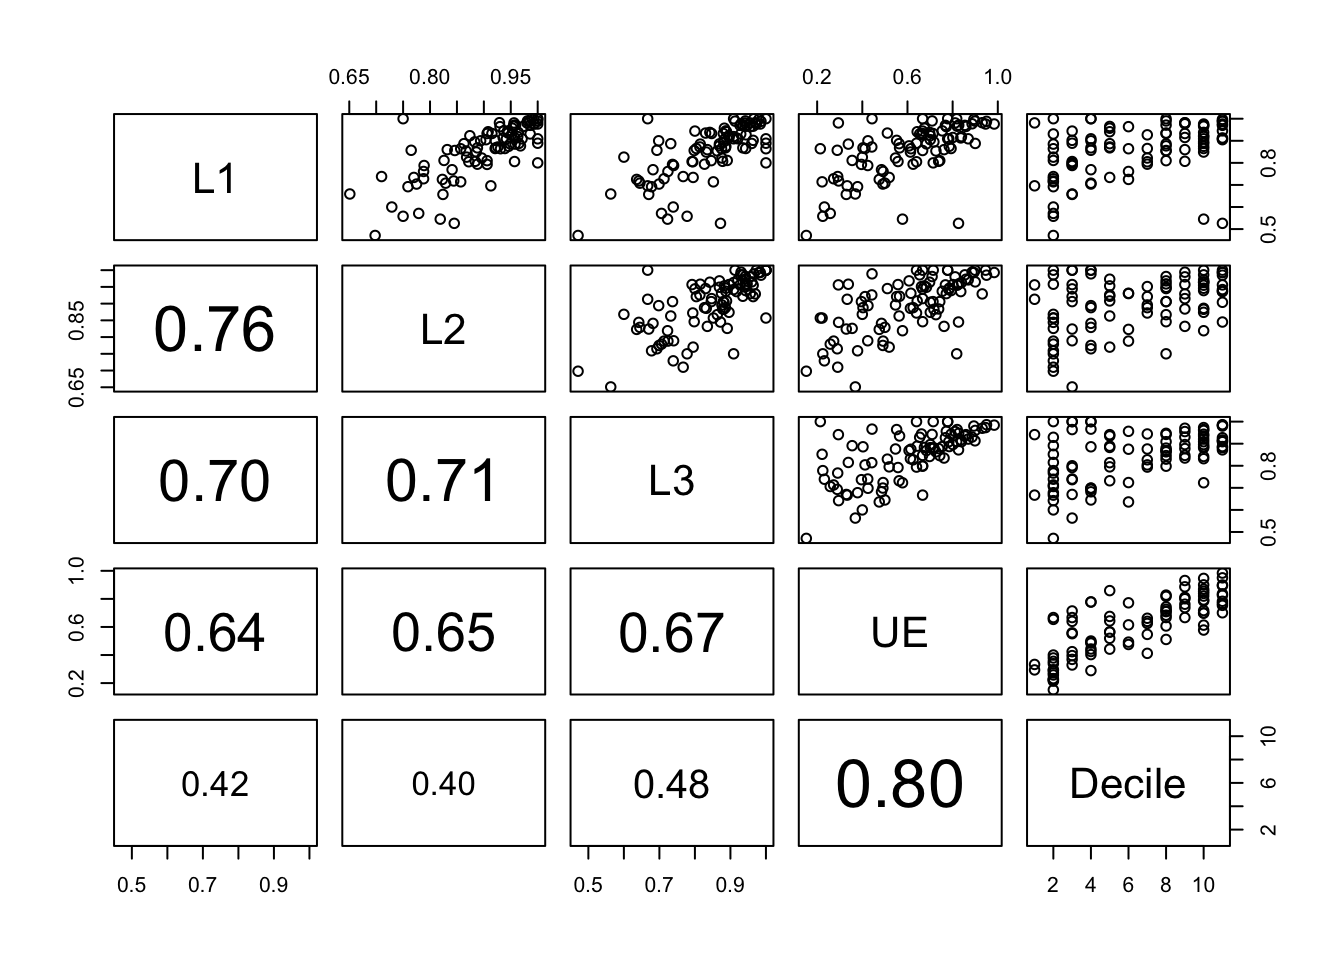
\includegraphics{ReportDraft_files/figure-latex/pairs-1.pdf}
\caption{\label{fig:pairs}Pairs plot for NCEA data on Auckland schools.}
\end{figure}

\begin{figure}[htbp]
\centering
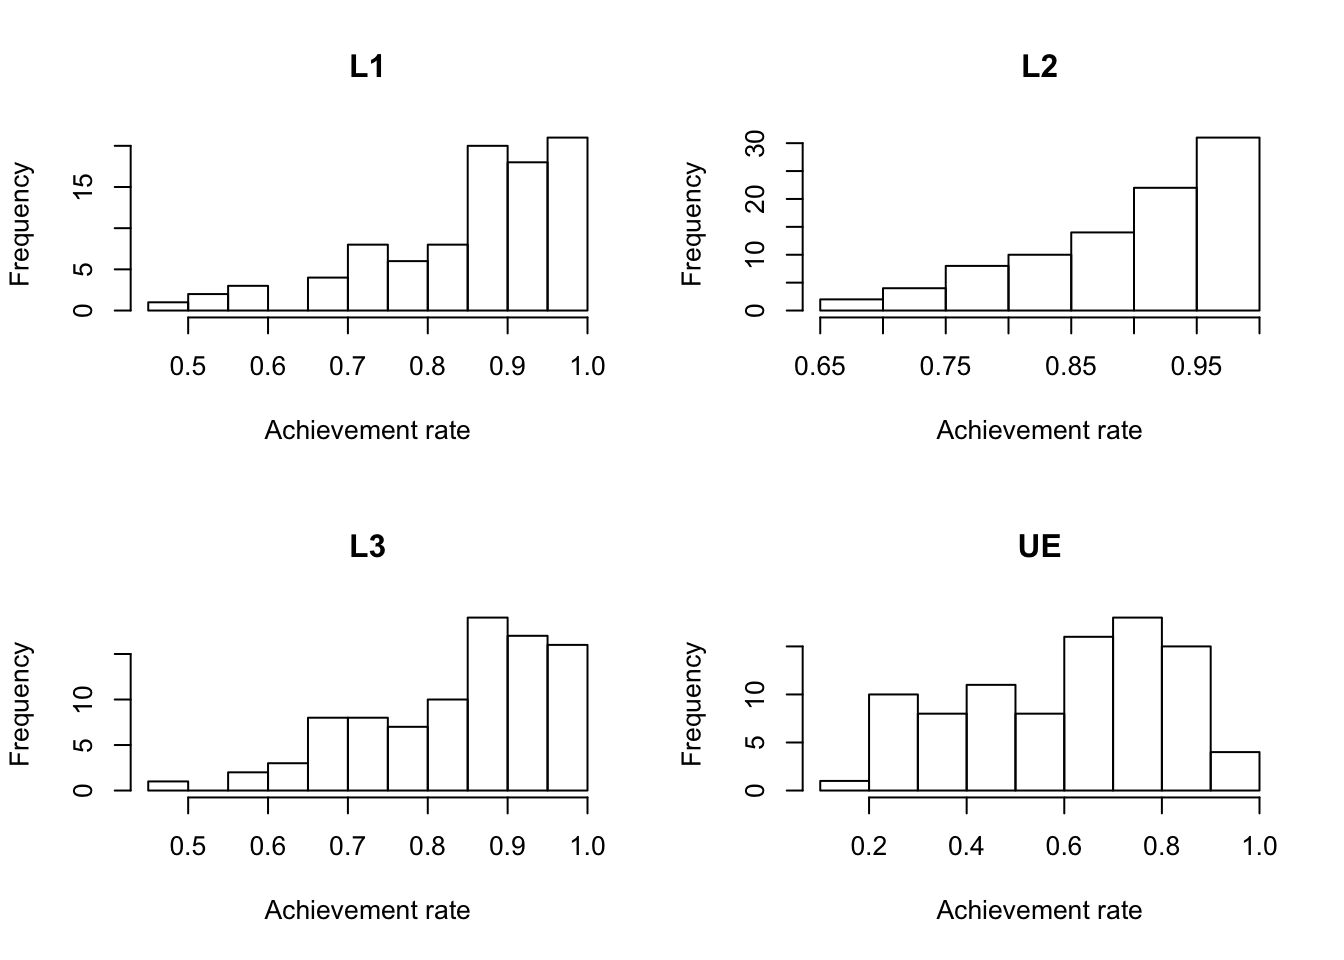
\includegraphics{ReportDraft_files/figure-latex/hists-1.pdf}
\caption{\label{fig:hists}Univariate distributions for NCEA data on Auckland
schools.}
\end{figure}

\section{Multivariate visual
representations}\label{multivariate-visual-representations}

The pairs plot in Figure \ref{fig:pairs} provided a glimpse into the
multivariate distribution of achievement rates across the four
qualification levels. The parallel coordinates plot in Figure
\ref{fig:pcpAkl} allows us to further compare the multivariate
distributions of achievement rates for different decile groups, as well
as identify high dimensional clusters and outliers, if they exist.

The ordering of axes in a parallel coordinates plots (PCP) greatly
affects the quality of the graphical analysis, hence interactivity that
enables reordering of axes is recommended Unwin (2015). In the case of
the NCEA data, the natural ordering of the four qualification levels by
difficulty, conincides with the recommendation from Cook and Swayne
(2007) to order the axes based on correlation. In addition, Unwin (2015)
highlights the layering of colours also needs to be considered
carefully, since the last group assigned a colour will dominate the
other lines.

The positive relationships previously identified in the pairs plot,
should translate to approximately horizontal lines between the parallel
axes in the PCP, as opposed to sloped or ``criss-crossed'' lines for
negative correlation. The static plot in Figure \ref{fig:pcpAkl}
questions whether the positive relationships hold true for Auckland
schools with low achievement rates and in some decile groups. In
particular, there appears to be a negative relationship between
achievement rates at L3 and UE for many schools. The achievement rates
for UE are clearly the most variable.

The higher decile schools in Auckland appear to dominate the high
achievement rates across all qualification levels, while lower decile
schools are less consistent with each other in terms of their
performance across the levels. Although there are only 91 observations
(lines), it is quite difficult to identify even ``ball park
boundaries'', on the 10-point decile scale, to distinguish between
``higher'' and ``lower'' decile schools when describing possible
patterns.

\begin{figure}[htbp]
\centering
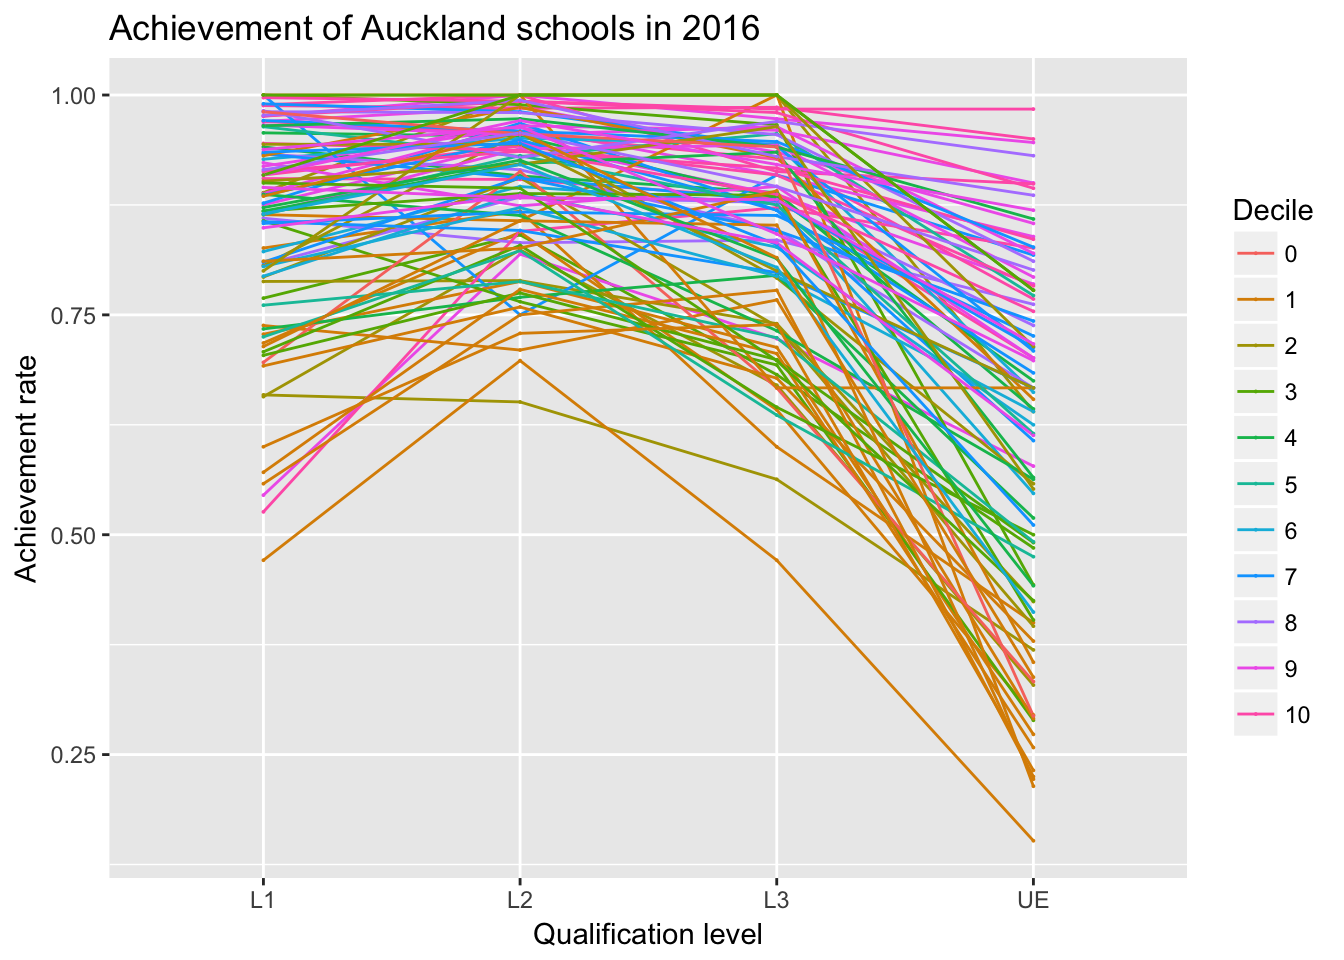
\includegraphics{ReportDraft_files/figure-latex/pcpAkl-1.pdf}
\caption{\label{fig:pcpAkl}Parallel coordinates plot for NCEA data on
Auckland schools.}
\end{figure}

The following two plots demonstrate how alpha blending can help minimise
the effects of overplotting as the number of observations increase. It
is easier to check whether the patterns identified in Auckland schools
extend to the 408 schools across New Zealand, using Figure
\ref{fig:pcpAlpha} where alpha blending is applied, rather than Figure
\ref{fig:pcpNZ}. The performance of high achieving lower decile schools
is less ``drowned out'' by the dominance of their higher decile
counterparts, when alpha blending is used. Figure \ref{fig:pcpAlpha}
reveals a group of schools converging at 100\% achievement for L3, but
with varying levels of success at L2 and UE. It would be of interest to
compare the achievement rates of these schools across the qualification
levels. Similarly, we would be interested in tracking the performance of
the school with the lowest achievement rate at L1. The school appears to
make a convincing recovery in performance at L2, but it is impossible to
follow its progress further in a static PCP due to overplotting.
Interactive techniques will be later used to explore these points of
interest.

\begin{figure}[htbp]
\centering
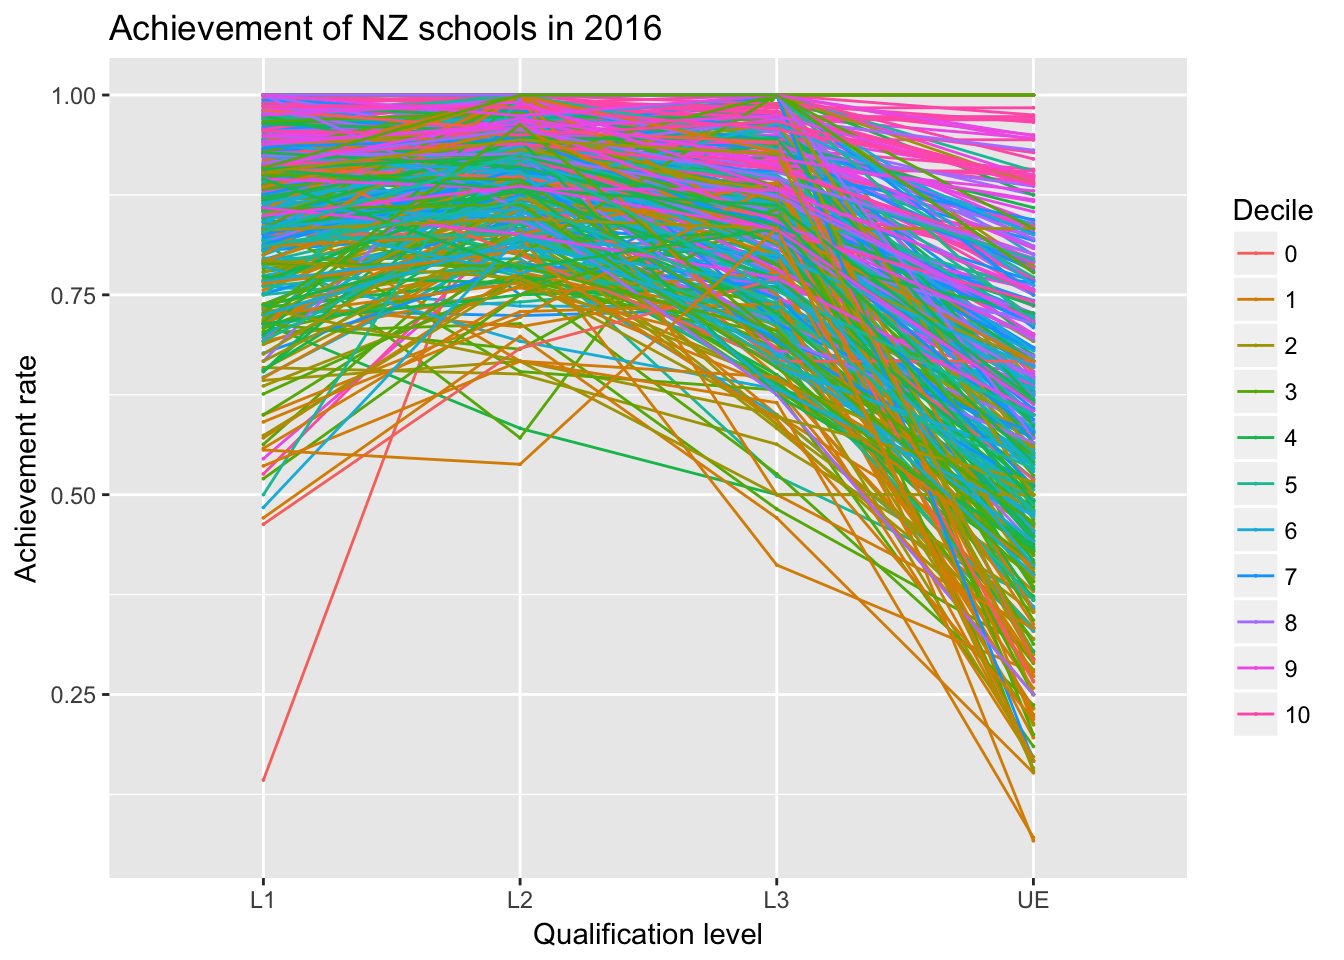
\includegraphics{ReportDraft_files/figure-latex/pcpNZ-1.pdf}
\caption{\label{fig:pcpNZ}Parallel coordinates plot for New Zealand schools,
without alpha blending.}
\end{figure}

\begin{figure}[htbp]
\centering
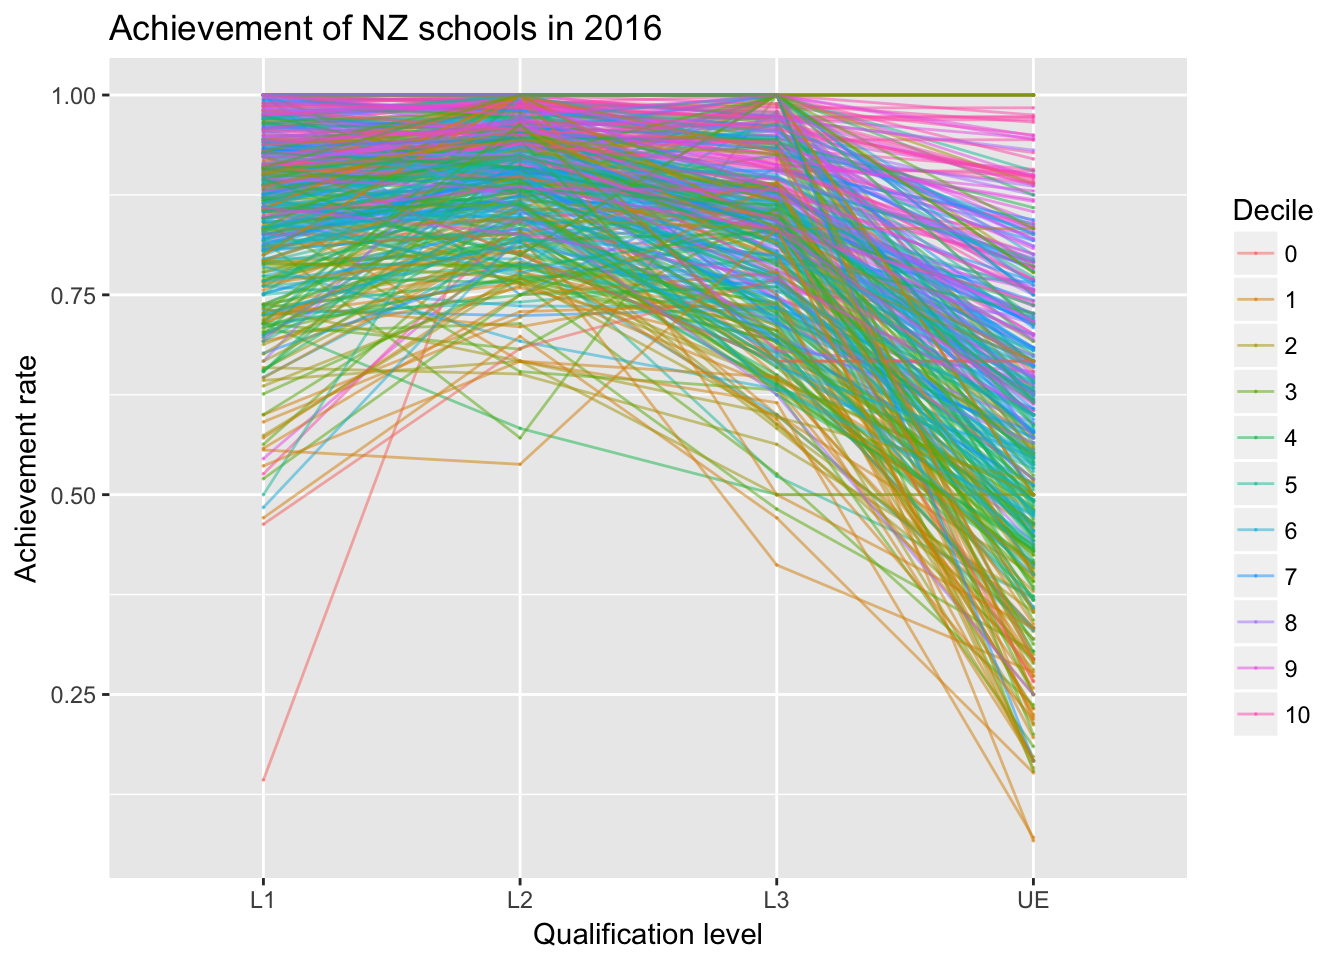
\includegraphics{ReportDraft_files/figure-latex/pcpAlpha-1.pdf}
\caption{\label{fig:pcpAlpha}Parallel coordinates plot for New Zealand
schools, with alpha blending.}
\end{figure}

\section{Design of visuals}\label{design-of-visuals}

As previously discussed in Section \ref{scaling}, scaling affects the
structures highlighted by a PCP. Figure @ref(fig:pcp\_scale)
demonstrates how different scale choices can be interactively explored.

\begin{figure}[center]
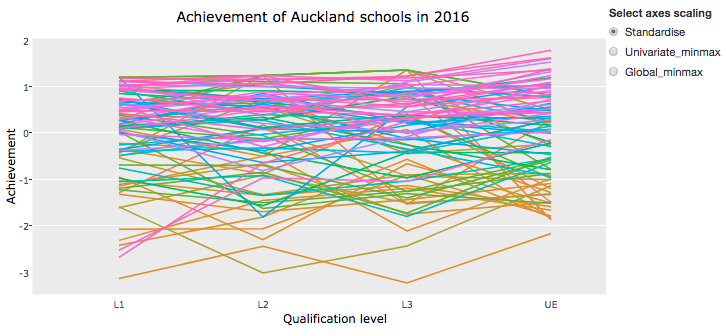
\includegraphics[width=700px]{files/pcp_scale} \caption{Interactively exploring the effect of scaling on a PCP.}(\#fig:pcp_scale)
\end{figure}

Standardising the achievement rates creates a PCP for comparison between
the performance of schools. Similarly, rescaling each variable to range
from 0 to 1 (achieved by \texttt{Univariate\_minmax}) focuses on ranking
the cases and comparing performance within qualification levels.
Patterns of achievement across the qualification levels are of interest,
hence scaling using the global minimum and maximum values, used in
Figures \ref{fig:pcpAkl} to \ref{fig:pcpAlpha}, will be retained in
further analysis. However being able to compare the effects of scaling
quickly and dynamically, highlights the common patterns that can be
identified. In particular, the dominance of the higher decile schools
and the inconsistent performance across qualification levels for some
deciles.

\begin{boxed}
Interactivity allows important decisions, like the choice of scale, to
be considered carefully. Different scales can be examined quickly and
dynamically.
\end{boxed}

\section{Leveraging static plots with
interactivity}\label{leveraging-static-plots-with-interactivity}

Although one of the strengths of a PCP is in identifying multivariate
features, such as outliers (Cook and Swayne 2007), the static plots in
Figures \ref{fig:pcpNZ} and \ref{fig:pcpAlpha} do not allow these
features to be explored, due to overplotting. The use of colour and
interactive techniques are recommended for maximising the effectiveness
of a PCP. Venables and Ripley (2002) argue parallel coordinate plots are
``often too `busy' without means of interaction'' (p.315). The
interactive filtering feature in Figure \ref{fig:pcpInt} addresses the
problem of overplotting by allowing the user to isolate the distribution
of each decile group (via a double-click on the legend). Furthermore,
using the mouse to drag-and-select nodes on the parallel axes, brushes
and links the acheivement rates of individual schools across all
qualification levels. Lastly the hovering tooltip enables instant
identification of indvidual schools by name.

\begin{boxed}
Interactive filtering alleviates issuses with overplotting when the
number of observations increase.
\end{boxed}

\hypertarget{4e075bed8bf0}{}

\label{fig:pcpInt}Parallel coordinates plot with interactivity.

Figure \ref{fig:pcpOut} demonstrates the use of interactive techniques
to explore the outlier at L1, previously identified in Figure
\ref{fig:pcpAlpha}. The tooltip identifies the school and the linked
brushing reveals that despite its poor performance at L1, the school had
100\% achievement rates at L2 and L3.

\begin{boxed}
Brushing within an individual plot overcomes overplotting to highlight
features of interest.
\end{boxed}

\begin{figure}[center]
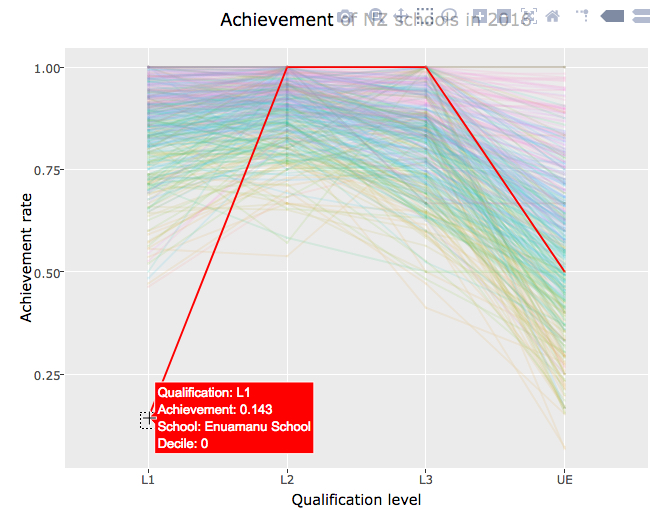
\includegraphics[width=700px]{files/pcp_outlier} \caption{Linked brushing to examine outliers.}\label{fig:pcpOut}
\end{figure}

Cook and Swayne (2007) describe how linked brushing enables dynamic
database querying and direct comparisons between subsets of data and the
general distribution. Figure \ref{fig:pcpL3} illustrates how brushing
the point where L3=100\% on the interactive PCP, highlights the extent
of the variability in performance at the other qualification levels.
Surprisingly, the distribution of UE achievement rates for schools with
100\% achievement at L3, is just as spread out as the overall
performance of New Zealand schools in the dataset. Many of these schools
also obtained 100\% achievement rates at L2, but again there is
surprisingly variable success at L1.

\begin{figure}[center]
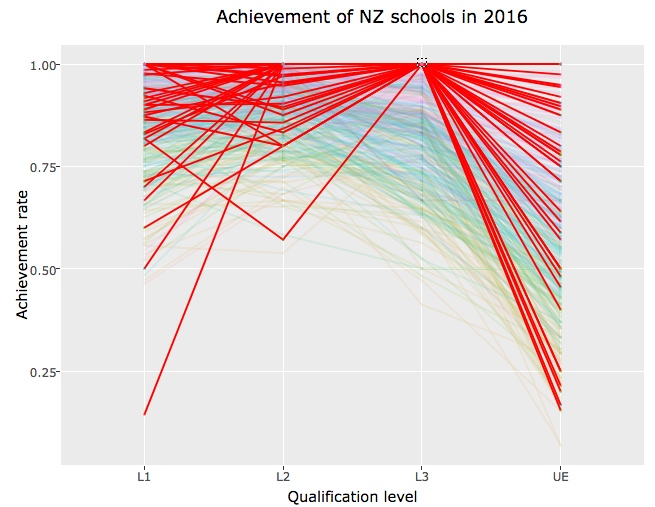
\includegraphics[width=700px]{files/pcp_L3} \caption{Linked brushing to subset groups of interest.}\label{fig:pcpL3}
\end{figure}

The query made via linked brushing in Figure \ref{fig:pcpL3} is similar
to subsetting the data using the code shown below. A summary could be
used to examine the performance of the subset of 42 schools across the
other qualifications, but making sense of this summary would required
comparison with statistics for the whole dataset. Furthermore the
summary hides the unusual performance of individual schools at certain
qualification levels. The interactive techniques allowed us to gain
insights about the NCEA data, that would have been difficult to
ascertain from static plots or numeric summaries alone.

\begin{Shaded}
\begin{Highlighting}[]
\NormalTok{L3all_achieve <-}\StringTok{ }\NormalTok{nzqa[nzqa$L3==}\DecValTok{1}\NormalTok{, }\KeywordTok{c}\NormalTok{(}\StringTok{"L1"}\NormalTok{, }\StringTok{"L2"}\NormalTok{, }\StringTok{"UE"}\NormalTok{)]}
\KeywordTok{nrow}\NormalTok{(L3all_achieve)}
\end{Highlighting}
\end{Shaded}

\begin{verbatim}
## [1] 42
\end{verbatim}

\begin{Shaded}
\begin{Highlighting}[]
\KeywordTok{summary}\NormalTok{(L3all_achieve)}
\end{Highlighting}
\end{Shaded}

\begin{verbatim}
##        L1               L2               UE        
##  Min.   :0.1430   Min.   :0.5710   Min.   :0.1540  
##  1st Qu.:0.8407   1st Qu.:0.9073   1st Qu.:0.5000  
##  Median :0.9260   Median :1.0000   Median :0.7700  
##  Mean   :0.8848   Mean   :0.9463   Mean   :0.7025  
##  3rd Qu.:1.0000   3rd Qu.:1.0000   3rd Qu.:0.9380  
##  Max.   :1.0000   Max.   :1.0000   Max.   :1.0000
\end{verbatim}

\begin{boxed}
Linked brushing and tooltip identification, allow fast querying of
unusual patterns, groups and/or individuals. The instant visual feedback
is especially useful for exploratory analysis.
\end{boxed}

However the ease and effectiveness of linked brushing can also be
affected by overplotting. Figure \ref{fig:pcpBusy} demonstrates how an
attempt to use persistent brushing to identify the UE success rate of
the school with 100\% achievement at L3, but unusually low performance
at L2, resulted in accidentally brushing an observation with a similar
L2 achievement rate. The \textbf{plotly} R package used in Figure
\ref{fig:pcpInt} allows only the nodes of the PCP to be brushed. The
\textbf{ggobi} GUI applies the same drag-and-select motion to brush both
points and lines on a PCP (Cook and Swayne 2007). This greater
flexibility would have avoided the issues caused by overplotting in this
case, but some of the challenges of large datasets for static graphical
displays will persist, even with interactive techniques. In particular
the speed of rendering plots for large datasets determines whether the
techinques can be applied ``fast enough to be considered interactive''
(Unwin 2015, 27:20).

\begin{boxed}
The effectiveness of interactive techniques for large datasets will be
affected by rendering delays and limitations imposed by plot size and
resolution.
\end{boxed}

\begin{figure}[center]
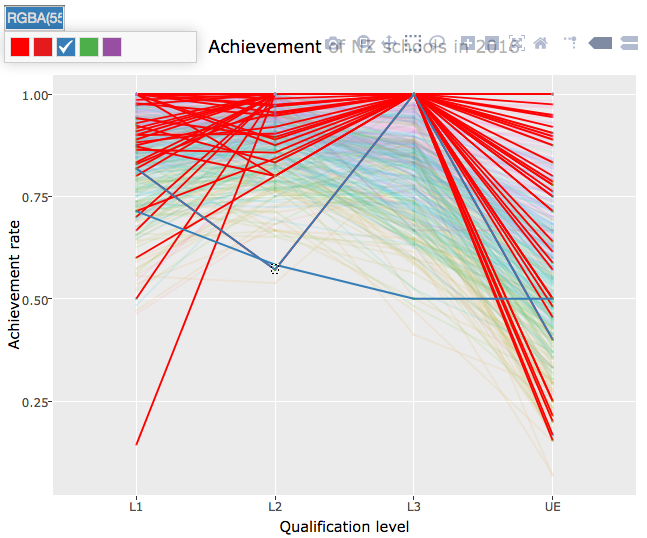
\includegraphics[width=700px]{files/pcp_busy} \caption{Accuracy of brushing is affected by overplotting.}\label{fig:pcpBusy}
\end{figure}

The PCP in Figure \ref{fig:pcpAkl} suggests that patterns of performance
across decile groups, if they exist, are difficult to distinguish at the
multivariate level for Auckland schools. Hence principal component
analysis (PCA) was applied to further examine the underlying
multivariate structures. A plot of the first two principal components of
the \textbf{Auckland schools} dataset is shown in Figure
\ref{fig:pcaAkl}. Line segments with labels of the original variable
names are used to represent the loadings of the principal components.
The loadings are the contributions of each variable to the linear
combinations that define the principal components (Venables and Ripley
2002). Since all four variable axes are orientated horizontally in the
same direction, the first principal component reflects the schools'
general performance across all four qualification levels. The vertical
separation between the UE axis and the remaining axes, indicates that
the second principal component contrasts performance in UE against the
other qualifications. Not surprisingly the plot shows more spread across
the first principal component since it explains a much greater
proportion of the variation in the data. The first principal component
reveals a division between the majority of schools and a smaller group,
that is positioned away from the variable axes shown. The decile of the
schools is represented by the colour and plotting symbol. The smaller
group of schools appear to be decile five and below, except for one
decile nine school. There is also a decile ten school that appears to be
unusual when examining both principal components. The use of colour
highlights the remaining decile nine and ten schools as similar in
performance, as weighted by the principal components. On the other hand,
schools from the other deciles seem to be more spread out from each
other in the PCA plot.

\begin{figure}[htbp]
\centering
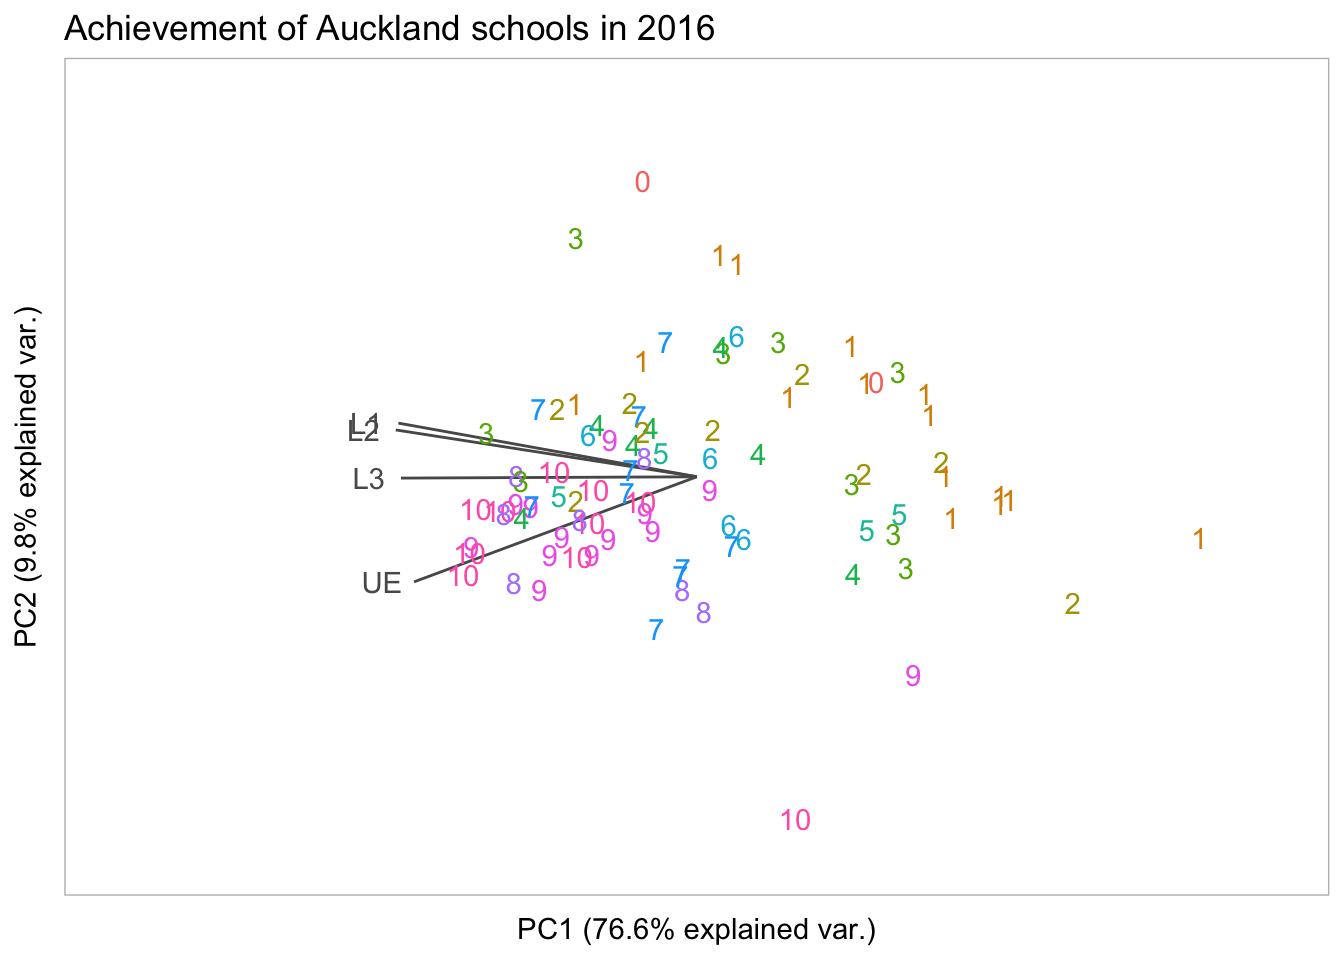
\includegraphics{ReportDraft_files/figure-latex/pcaAkl-1.pdf}
\caption{\label{fig:pcaAkl}First two principal components for Auckland
schools}
\end{figure}

The principal components plot in Figure \ref{fig:pcaAkl} provided a view
of the multivariate distribution of the Auckland schools dataset that
was less easily affected by overplotting than a static PCP. Hence
refinements on observations were possible. From the parallel coordinate
plots we observed that ``higher'' decile schools performed more
consistently with each other and dominating across the four
qualification levels, but it was difficult to quantify the decile ``cut
off'' for such schools. The PCA suggests these schools are the decile
nine and ten Auckland schools, with the exception of two schools. Again
interactive tooltips enable instant identification of these two unusual
observations, in Figure \ref{fig:pcaInt}.

Furthermore the two plots in Figure \ref{fig:pcaInt} are interactively
linked by brushing. Individual or groups of points in the PCA plot can
be brushed via a drag-and-select motion using the mouse. The ``Lasso
Select'' option can be activated from the hovering menu on the top right
hand corner, if the region of points to be selected is irregular rather
than rectangular. The original achievement rates of the selected schools
will be highlighted in the PCP, while the lines for the unselected
schools will be dimmed. Similarly brushing on the nodes of the PCP
highlights the observations on the PCA plot.

\hypertarget{4e0727f1afe2}{}

\hypertarget{4e074e33cbe5}{}

\label{fig:pcaInt}First two principal components for Auckland schools with
interactivity.

Figure \ref{fig:brushGroup} demonstrates the use of the lasso brush to
highlight the original variable values of the central group of points in
the PCA plot. The linked brushing and tooltip identification reveals
that these Auckland schools have at least 80\% achievement rates at all
four qualification levels, except for UE. We are also able to identify
the only decile one school in this group.

\begin{figure}[center]
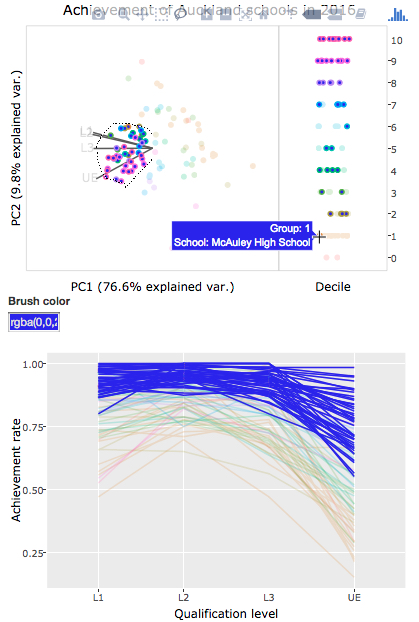
\includegraphics[width=500px]{files/link_group} \caption{Brushing a central group of points in the PCA plot links with the decile and achievement rates of the selected schools.}\label{fig:brushGroup}
\end{figure}

In a similar manner to Figure \ref{fig:pcpBusy}, persistent brushing can
be applied with different colours to further explore the multivariate
features revealed by the PCA. The three outliers brushed in the PCA plot
are at two extremes. Comparing their achievement rates on the PCP helps
to explain why they are unusual in different ways. Two of the outliers
had consistently high performance at the first three qualification
levels, but there was a drastic drop in the UE achievement rate.
Although, as previously observed, lower performance at UE was shared by
the Auckland schools in general, the large differences between the two
schools' achievement rates for UE and the remaining qualification
levels, are still unexpected. The single outlier at the other extreme of
the PCA plot, defies the general trend. Its L1 achievement rate was
inconsistently lower than the other qualification levels, rather its UE
rate. Although all three schools had unusual performance compared to
Auckland schools in general, the inconsistencies in their performance
differed. The linked brushing enabled us to further investigate the
differences in ``unusualness'' and it also highlights how the
multivariate outliers identified in the PCA are hidden in the PCP.

\begin{boxed}
The insights into multidimensional data structures gained from
individual static plots were extended when linked brushing was applied.
\end{boxed}

\begin{figure}[center]
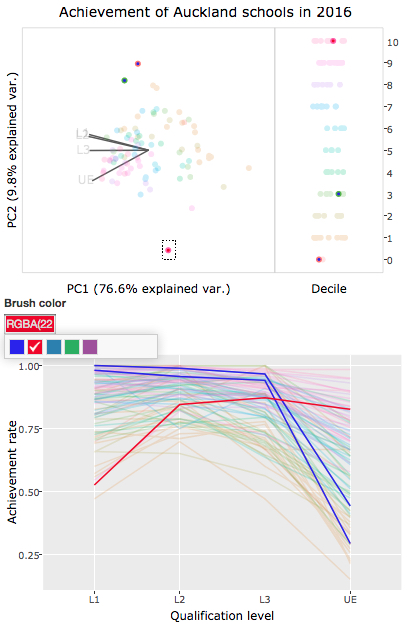
\includegraphics[width=500px]{files/link_outPCA} \caption{Brushing outliers on the PCA plot identifies inconsistent patterns of achievement on the PCP.}\label{fig:brushOutPCA}
\end{figure}

Initiating the linked brushing from the PCP is also useful. Figure
@ref(fig: brushOutPCP) confirms the outliers visible in the PCP are also
identified as outliers in the PCA. The PCP highlights schools that have
unusually low achievement rates at a particular qualification level,
while the outliers from the PCA encompasses these schools, as well as
those that are unusual in terms of patterns of performance. Unwin (2015)
emphasises the importance of generating a variety of visual when
applying graphical data analysis. The different views provided reveal
different aspects of the data.

\begin{figure}[center]
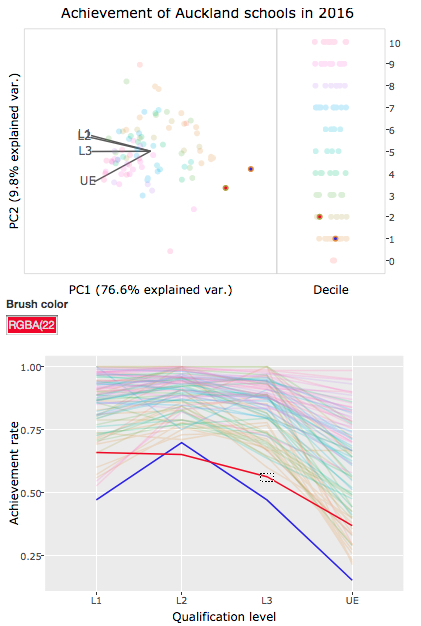
\includegraphics[width=500px]{files/link_outPCP} \caption{Brushing outliers on the PCP confirms their status as also outliers in the PCA plot.}\label{fig:brushOutPCP}
\end{figure}

\section{Interactive analyses}\label{interactive-analyses}

The NZQA indicator of a ``small'' cohort was at a very low threshold of
fewer than five candidates at any qualification level. Hence information
on the number of Year 11, 12 and 13 students at each school in 2016, was
sourced from the New Zealand government website, Education
Counts.\footnote{Data retrieved from
  \url{https://www.educationcounts.govt.nz/__data/assets/excel_doc/0005/152609/Student-rolls-by-School-2010-2016.xlsx}}
The minimum cohort size for the three senior year levels will be used as
indicator of whether the NCEA achievement rates were based on small
sample sizes. The website also provided information on the ethnic
composition of the New Zealand schools in terms of six general
categories: Maori, Pasifika, Asian, Middle Eastern/Latin
American/African (MELAA), Other and European/Pakeha. Hence the merged
dataset contains additional information on region, type, total roll
size, proportions of students in the six ethnic categories and a minimum
cohort size based on the number of students at the senior levels.

\begin{table}

\caption{\label{tab:unnamed-chunk-14}The first few observations from the merged **NCEA** dataset. The data consists of ten real-valued variables, two discrete variables and three categorical variables.}
\centering
\begin{tabular}[t]{lrrrrlllrrrrrrrr}
\toprule
School & L1 & L2 & L3 & UE & Decile & Region & Type & Total & Maori & Pasifika & Asian & MELAA & Other & EuropeanPakeha & Min.Cohort\\
\midrule
Akaroa Area School & 1.000 & 0.800 & 1.000 & 1.000 & 8 & Christchurch/Canterbury & Composite (Year 1-15) & 144 & 0.20 & 0.00 & 0.01 & 0.03 & 0.00 & 0.76 & 6\\
Al-Madinah School & 0.889 & 1.000 & 1.000 & 0.640 & 2 & Auckland & Composite (Year 1-15) & 530 & 0.00 & 0.00 & 0.93 & 0.06 & 0.01 & 0.00 & 18\\
Albany Senior High School & 0.905 & 0.904 & 0.882 & 0.701 & 10 & Auckland & Secondary (Year 9-15) & 759 & 0.08 & 0.01 & 0.19 & 0.08 & 0.02 & 0.62 & 246\\
\bottomrule
\end{tabular}
\end{table}

Figure \ref{fig:pcaSize} explores the effect of sample size on the
principal component analysis. The interactive slider subsets the schools
according to their minimum cohort size before PCA is performed. The
effect of varying the sample size can be dynamically viewed by selecting
the ``play'' icon on the slider, as shown in Figure \ref{fig:pcaSize}.

\begin{figure}[center]
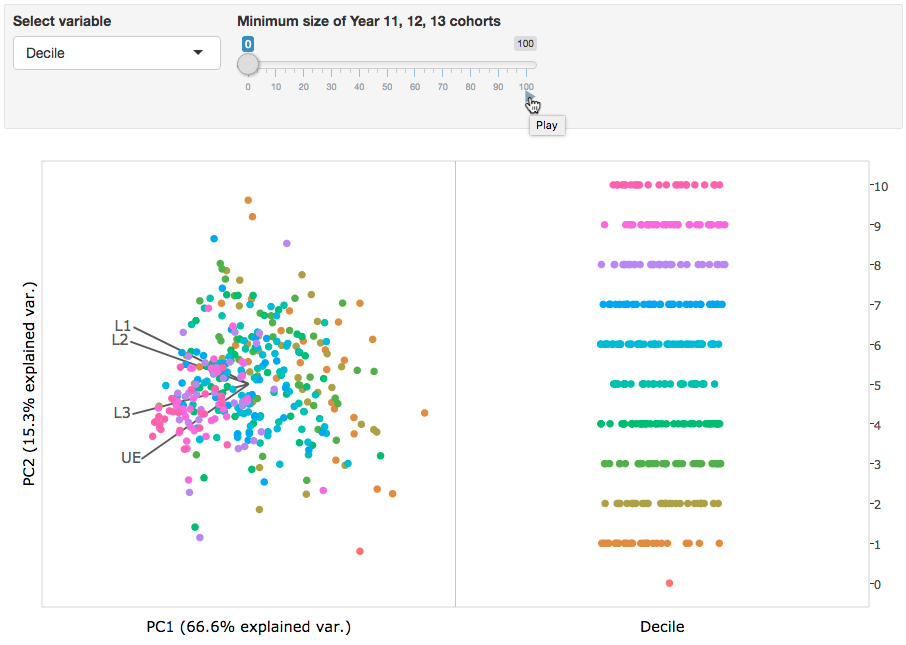
\includegraphics[width=500px]{files/pca_shiny0} \caption{Interactivity to explore the effect of sample size. See <https://shanl33.shinyapps.io/ncea/>.}\label{fig:pcaSize}
\end{figure}

The pattern previously noted for Auckland schools, where decile nine and
ten schools were more consistent with each other in performance than the
other deciles, appears to hold for New Zealand schools in general. Not
surprisingly, as the minimum cohort size increases, the spread in the
PCA plot decreases and the first principal component is able to explain
more of the variation in the data. The axes for the original variables,
reflecting the loadings of the principal components, remain reasonably
consistent. The first principal component generally measures overall
performance across the four qualification levels, while the second
component contrasts L1 and L2 preformance against L3 and UE.

\begin{boxed}
Dynamic visualisation allows multiple analyses to be computed and
compared quickly. The flexibility of being able to pause animations
allows closer examination of details, as the need arises.
\end{boxed}

The interactive drop-down menu also allows us to quickly verify whether
there are any underlying relationships between achievement rates and
demographics other than decile, that are worth further investigation.
Although the other demographic variables did not reveal any further
insight, the ease with which these additional variables could be
interactively linked to the PCA plot, justified their inclusion in the
exploratory data analysis. Enabling the interactive drop-down menu in
Figure \ref{fig:pcaSize} involved adding the following single command to
the code.

\begin{Shaded}
\begin{Highlighting}[]
\KeywordTok{selectInput}\NormalTok{(}\StringTok{"group"}\NormalTok{, }\StringTok{"Select variable"}\NormalTok{, }\DataTypeTok{choices=}\KeywordTok{as.list}\NormalTok{(}\KeywordTok{colnames}\NormalTok{(nzqa.sch)[}\DecValTok{6}\NormalTok{:}\DecValTok{15}\NormalTok{]), }\DataTypeTok{selected=}\StringTok{"Decile"}\NormalTok{)}
\end{Highlighting}
\end{Shaded}

\begin{boxed}
When interactive techniques can be applied with ease, the trade-off
between the effort required to implement the techniques and the level of
insight gained, is generally favourable.
\end{boxed}

The ease with which the other demographic variables could be
investigated in Figure \ref{fig:pcaSize} also emphasises the value of
applying interactive techniques in exploratory data analysis. Cook and
Swayne (2007) highlights how interactive data visualisation supports
``slipping out of dead-ends and chasing down new leads'' (p.11).

\begin{boxed}
Applying interactive data visualisation encourages further exploration
of the data. Questions are addressed quickly and more questions arise
from probing the data with interactive techniques.
\end{boxed}

\section{Viewing the data space}\label{viewing-the-data-space}

Wickham, Cook, and Hofmann (2015) applied tours to encourage the
visualisation of statistical models in the data space. They demonstrated
how linked brushing between visual representations of summary statistics
and displays of models, allows subsets of models to be compared.

\begin{figure}[center]
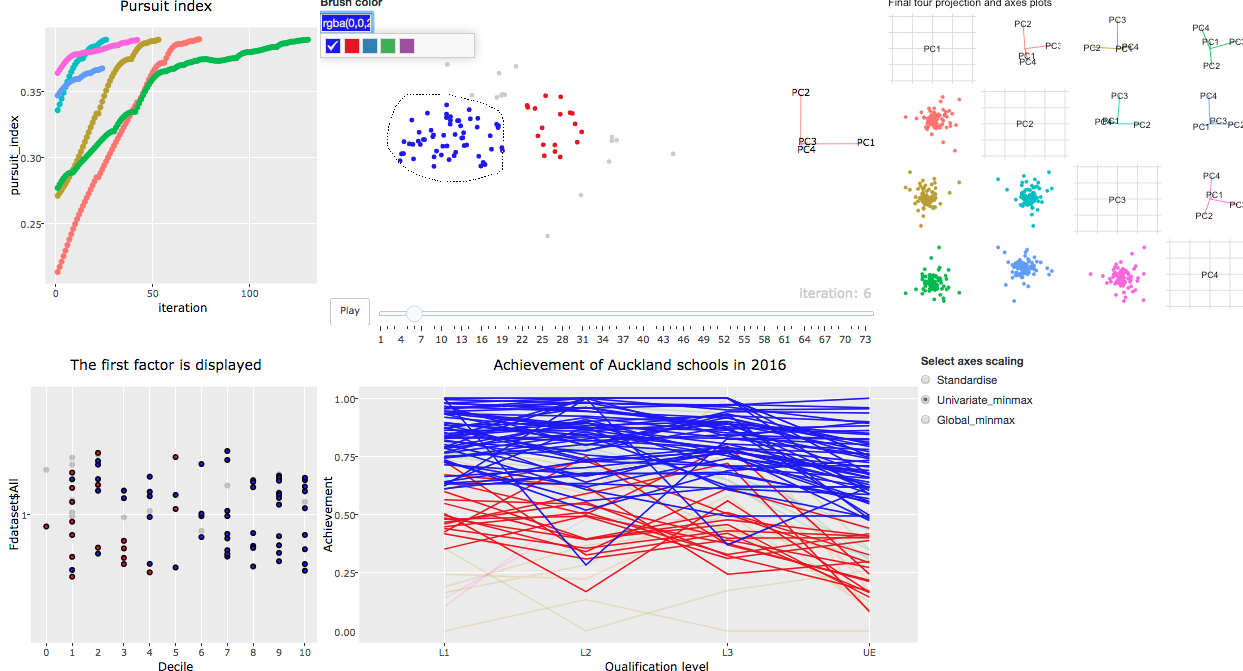
\includegraphics[width=500px]{files/finalApp} \caption{Guided tour of achievement rates for Auckland schools. See <https://shanl33.shinyapps.io/nceaTour/>.}\label{fig:nceaTour}
\end{figure}

\begin{boxed}
Interactive techniques like linked brushing and tours, allow multiple
views of the data to be viewed at the same time. Consequently leading to
a more thorough exploration of data structures.
\end{boxed}

\hypertarget{refs}{}
\hypertarget{ref-Cook}{}
Cook, Dianne, and Deborah F. Swayne. 2007. \emph{Interactive and Dynamic
Graphics for Data Analysis with R and Ggobi}. 1st ed. Springer
Publishing Company, Incorporated.

\hypertarget{ref-trelliscope}{}
Hafen, Ryan. 2017. ``Trelliscopejs.'' Accessed October 20.
\url{https://hafen.github.io/trelliscopejs/\#why_trelliscope}.

\hypertarget{ref-animint}{}
Hocking, Toby Dylan. 2017. ``Animint: Animated and Interactive Web
Graphics.'' \url{https://github.com/tdhock/animint}.

\hypertarget{ref-Lang}{}
Lang, Duncan Temple, and Deborah F Swayne. 2001. ``GGobi Meets R: An
Extensible Environment for Interactive Dynamic Data Visualization.'' In
\emph{Proceedings of Dsc}, 2.

\hypertarget{ref-Lawrence}{}
Lawrence, Michael, Hadley Wickham, Dianne Cook, Heike Hofmann, and
Deborah F. Swayne. 2009. ``Extending the GGobi Pipeline from R.''
\emph{Computational Statistics} 24 (2): 195--205.
doi:\href{https://doi.org/10.1007/s00180-008-0115-y}{10.1007/s00180-008-0115-y}.

\hypertarget{ref-crosstalk}{}
RStudio. 2017a. ``Authoring Crosstalk Widgets.'' Accessed October 23.
\url{https://rstudio.github.io/crosstalk/authoring.html}.

\hypertarget{ref-ggvis}{}
---------. 2017b. ``Interactivity.'' Accessed October 23.
\url{http://ggvis.rstudio.com/interactivity.html}.

\hypertarget{ref-shiny}{}
---------. 2017c. ``Shiny.'' Accessed October 23.
\url{https://shiny.rstudio.com/}.

\hypertarget{ref-plotly}{}
Seivert, Carson. 2017. ``Plotly: An Interactive Graphing Library for
R.'' rOpenSci. \url{https://github.com/ropensci/plotly}.

\hypertarget{ref-dendro}{}
Sievert, Carson. 2016. ``Hierarchial-Dendro.''
\url{https://vimeo.com/189670650}.

\hypertarget{ref-plotlyBook}{}
---------. 2017. \emph{Plotly for R}. Accessed October 24.
\url{http://ropensci.github.io/plotly/}.

\hypertarget{ref-mondrian}{}
Theus, Martin. 2017a. ``Mondrian - Interactive Statistical Data
Visualization in JAVA.'' Accessed October 23.
\url{http://www.theusrus.de/Mondrian/}.

\hypertarget{ref-tourdefrance}{}
---------. 2017b. ``Tour de France 100.'' \emph{Vimeo}. Accessed October
23. \url{https://vimeo.com/101951265}.

\hypertarget{ref-EDA}{}
Tukey, John W. 1977. \emph{Exploratory Data Analysis}. Addison-Wesley.

\hypertarget{ref-GDA}{}
Unwin, Antony. 2015. \emph{Graphical Data Analysis with R}. Vol. 27. CRC
Press.

\hypertarget{ref-Mass}{}
Venables, W. N., and B. D. Ripley. 2002. \emph{Modern Applied Statistics
with S}. Fourth. New York: Springer.
\url{http://www.stats.ox.ac.uk/pub/MASS4}.

\hypertarget{ref-blindfold}{}
Wickham, Hadley, Dianne Cook, and Heike Hofmann. 2015. ``Visualizing
Statistical Models: Removing the Blindfold.'' \emph{Statistical Analysis
and Data Mining: The ASA Data Science Journal} 8 (4). Wiley Subscription
Services, Inc., A Wiley Company: 203--25.
doi:\href{https://doi.org/10.1002/sam.11271}{10.1002/sam.11271}.

\hypertarget{ref-tourr}{}
Wickham, Hadley, Dianne Cook, Heike Hofmann, Andreas Buja, and others.
2011. ``Tourr: An R Package for Exploring Multivariate Data with
Projections.'' \emph{Journal of Statistical Software} 40 (2). Foundation
for Open Access Statistics: 1--18.

\hypertarget{ref-pipe}{}
Wickham, Hadley, Michael Lawrence, Dianne Cook, Andreas Buja, Heike
Hofmann, and Deborah F. Swayne. 2009. ``The Plumbing of Interactive
Graphics.'' \emph{Computational Statistics} 24 (2): 207--15.
doi:\href{https://doi.org/10.1007/s00180-008-0116-x}{10.1007/s00180-008-0116-x}.


\end{document}
